\chapter{MATERIAIS E MÉTODOS}\label{cap:metodologia}

Este capítulo descreve os materiais, a arquitetura, os procedimentos de desenvolvimento e os critérios de avaliação da plataforma experimental. Após a obtenção do modelo completo, é necessário obter a estabilização do sistema. Toda a estruturação e aplicação de técnicas de controle é realizada e validada no \textit{software} MATLAB/Simulink e posteriormente implementada no \textit{firmware} do controlador de voo. A validação do desempenho do sistema ocorre em ambiente interno, com o objetivo de reduzir riscos e permitir a coleta de dados confiáveis.

O objeto de estudo é um quadricóptero em configuração X destinado à validação de estabilização, telemetria e execução de missões simplificadas em ambiente interno. A arquitetura distribui responsabilidades entre um controlador de voo baseado em STM32F411 e um computador de missão Raspberry Pi Zero W. O STM32 executa as funções críticas de aquisição de sensores, estimação, controle, mistura de motores, geração de comandos DShot e \textit{failsafes}. O Raspberry Pi executa serviços de missão, comunicação em rede, roteamento e registro de telemetria; portanto, sua indisponibilidade não deve impedir o controlador de voo de entrar em estado seguro.

A comunicação entre as camadas é especificada como DroneLink (Seção~\ref{subsec:metodo_comunicacao}), uma camada própria do projeto executada sobre UART com enquadramento MAVLink 2. MAVLink é um protocolo de mensagens binárias desenvolvido para sistemas com recursos limitados e prevê identificação de sistemas/componentes, telemetria e mecanismos de integridade de mensagens \cite{koubaa2019,mavlinkguide}. No DroneLink, a rota calculada pelo módulo de planejamento é convertida em trechos de missão (\textit{legs}, na nomenclatura do protocolo: o deslocamento entre dois pontos consecutivos da rota) com identificação, confirmação, timeout e tratamento de duplicidade; o protocolo não substitui as proteções locais do controlador de voo, e o Raspberry Pi nunca envia PWM, DShot ou comandos diretos de motor.

\section{MATERIAIS E AMBIENTE DE EXECUÇÃO}\label{sec:materiais_ambiente}

Os componentes físicos da plataforma foram separados por função para facilitar a montagem, a inspeção visual e a rastreabilidade dos ensaios. A Figura~\ref{fig:componentes_principais} ilustra os principais módulos utilizados: controlador STM32F411, Raspberry Pi Zero W, unidade inercial BNO08X, sensor MicoAir MTF-01, ESC, motores, hélices, estrutura e elementos de alimentação. As imagens servem para identificar fisicamente os itens descritos no Quadro~\ref{qua:componentes}; especificações elétricas, versões e parâmetros de uso permanecem registrados no texto e nos quadros.

\newcommand{\componente}[2]{%
    \begin{minipage}[t]{0.30\textwidth}
        \centering
        \parbox[c][3.0cm][c]{\linewidth}{%
            \centering
            \includegraphics[
                width=\linewidth,
                height=2.9cm,
                keepaspectratio
            ]{#1}%
        }
        \par\vspace{0.08cm}
        {\footnotesize #2\par}
    \end{minipage}%
}

\begin{figure}[H]
    \centering
    \caption{Principais componentes físicos da plataforma experimental.}
    \label{fig:componentes_principais}

    \noindent
    \componente
        {images/hardware/STM32.png}
        {Controlador STM32F411}
    \hfill
    \componente
        {images/hardware/RPIZEROW16GB.png}
        {Raspberry Pi Zero W com SD de 16 GB}
    \hfill
    \componente
        {images/hardware/GY-BNO08X.png}
        {IMU BNO08X}

    \par\vspace{0.35cm}

    \noindent
    \componente
        {images/hardware/MTF01.png}
        {MicoAir MTF-01}
    \hfill
    \componente
        {images/hardware/ESC.jpg}
        {ESC 4 em 1}
    \hfill
    \componente
        {images/hardware/MOTOR-HELICE.png}
        {Motor e hélice}

    \par\vspace{0.35cm}

    \noindent
    \componente
        {images/hardware/GERPC.png}
        {Estrutura}
    \hfill
    \componente
        {images/hardware/BEC.png}
        {BEC}
    \hfill
    \componente
        {images/hardware/FONTECHAVEADA.png}
        {Fonte chaveada}

    \par\vspace{0.35cm}

    \noindent
    \hfill
    \componente
        {images/hardware/bateria_leao.png}
        {Bateria LiPo 3S}
    \hfill
    \componente
        {images/hardware/b6neo.png}
        {Carregador balanceador}
    \hfill\null

    \par\vspace{0.25cm}
    \begin{minipage}{0.95\textwidth}
        \centering
        \footnotesize Fonte: montagem elaborada pelos autores (2026); fotografias do Raspberry Pi Zero W e do conjunto motor--hélice dos autores; demais imagens obtidas por busca no Google Imagens.
    \end{minipage}
\end{figure}

O Quadro~\ref{qua:componentes} registra os principais materiais e especificações da plataforma experimental. Especificações comerciais são identificadas como tal; dados que dependem do exemplar físico, como a versão gravada do ESC, não são inferidos a partir de anúncios.

\begin{quadro}[htb]
\centering
\caption{Componentes da plataforma experimental.}
\label{qua:componentes}
\small
\renewcommand{\arraystretch}{1.3}
\begin{tabular}{
  |
  >{\raggedright\arraybackslash}p{3.2cm}
  |
  >{\raggedright\arraybackslash}p{10.8cm}
  |
}
\hline
\textbf{Função} & \textbf{Componente ou especificação} \\
\hline

Controlador de voo &
WeAct Studio MiniSTM32F4x1/Black Pill V3.1\newline
STM32F411CEU6, variante com HSE de 25~MHz\newline
Cortex-M4F, até 100~MHz, 512~kB de Flash e 128~kB de SRAM \cite{stm32f411ds}. \\[4pt]
\hline

Computador de missão &
Raspberry Pi Zero W v1.1\newline
BCM2835/ARMv6, 512~MB. \\[4pt]
\hline

IMU &
Módulo da família BNO08X; identificação específica a registrar por marcação física ou leitura do Product ID. \\[4pt]
\hline

Fluxo e altura &
MicoAir MTF-01; fluxo óptico, LiDAR ToF, UART 115200~bit/s e alimentação de 5~V segundo especificação do fabricante \cite{micoairmtf01}. \\[4pt]
\hline

Controlador de velocidade (ESC) &
Skystars KM55A II 4 em 1 (AM32 Turbo, 2024), AT32F421, 3S--6S, DShot300/DShot600/PWM. \\[4pt]
\hline

Propulsores (motores e hélices) &
4x Motores GEPRC SPEEDX2 2105.5, 2650KV. \newline
4x Hélices Gemfan D90-3. \\[4pt]
\hline

Estrutura &
Frame GEPRC CineLog35 V3, 3,5 polegadas. \\[4pt]
\hline

Energia &
1x Bateria Leão LB2200LP3, LiPo 3S (11,1~V), 2200~mAh, 30C.\newline
1x Micro BEC EXUAVRC/VTX BEC 2S--6S.\newline
1x capacitor de 680~$\mu$F, 35~V, baixo ESR. \\[4pt]
\hline

Carregador de bateria &
SkyRC B6neo 2, carregador balanceador para baterias LiPo. \\[4pt]
\hline

Fonte de bancada (Testes) &
Lumiville chaveada estabilizada bivolt, 12~V/50~A, 600~W; saída regulável de 12~V a 14~V. \\
\hline
\end{tabular}
\par\vspace{0.2cm}
\footnotesize Fonte: elaborado pelos autores (2026).
\end{quadro}

O módulo BNO08X implementa um hub de sensores com interface SH-2/SHTP. A biblioteca pública SH-2 disponibiliza, entre outros, \textit{reports} de acelerômetro, giroscópio, vetores de rotação e o acesso à identificação do produto \cite{sh2library}. A escolha do tipo de \textit{report}, sua taxa configurada e a latência efetivamente observada são registradas no ensaio, pois um limite publicado para uma saída específica não garante a mesma taxa para todas as saídas nem para a malha completa de controle \cite{bno08xdatasheet}.

A Figura~\ref{fig:prototipo_montado} apresenta a montagem final do protótipo em seis vistas, permitindo observar a distribuição dos módulos eletrônicos, da bateria, dos motores e das conexões sobre a estrutura. As indicações de direita e esquerda correspondem aos lados do próprio drone, considerando sua direção frontal, e não aos lados de quem observa a fotografia. A vista inferior evidencia a instalação do sensor de fluxo óptico e distância voltado para o solo.

\begin{figure}[htbp]
    \centering
    \caption{Montagem final do protótipo em seis vistas.}
    \label{fig:prototipo_montado}
    \begin{minipage}[t]{0.31\textwidth}
        \centering
        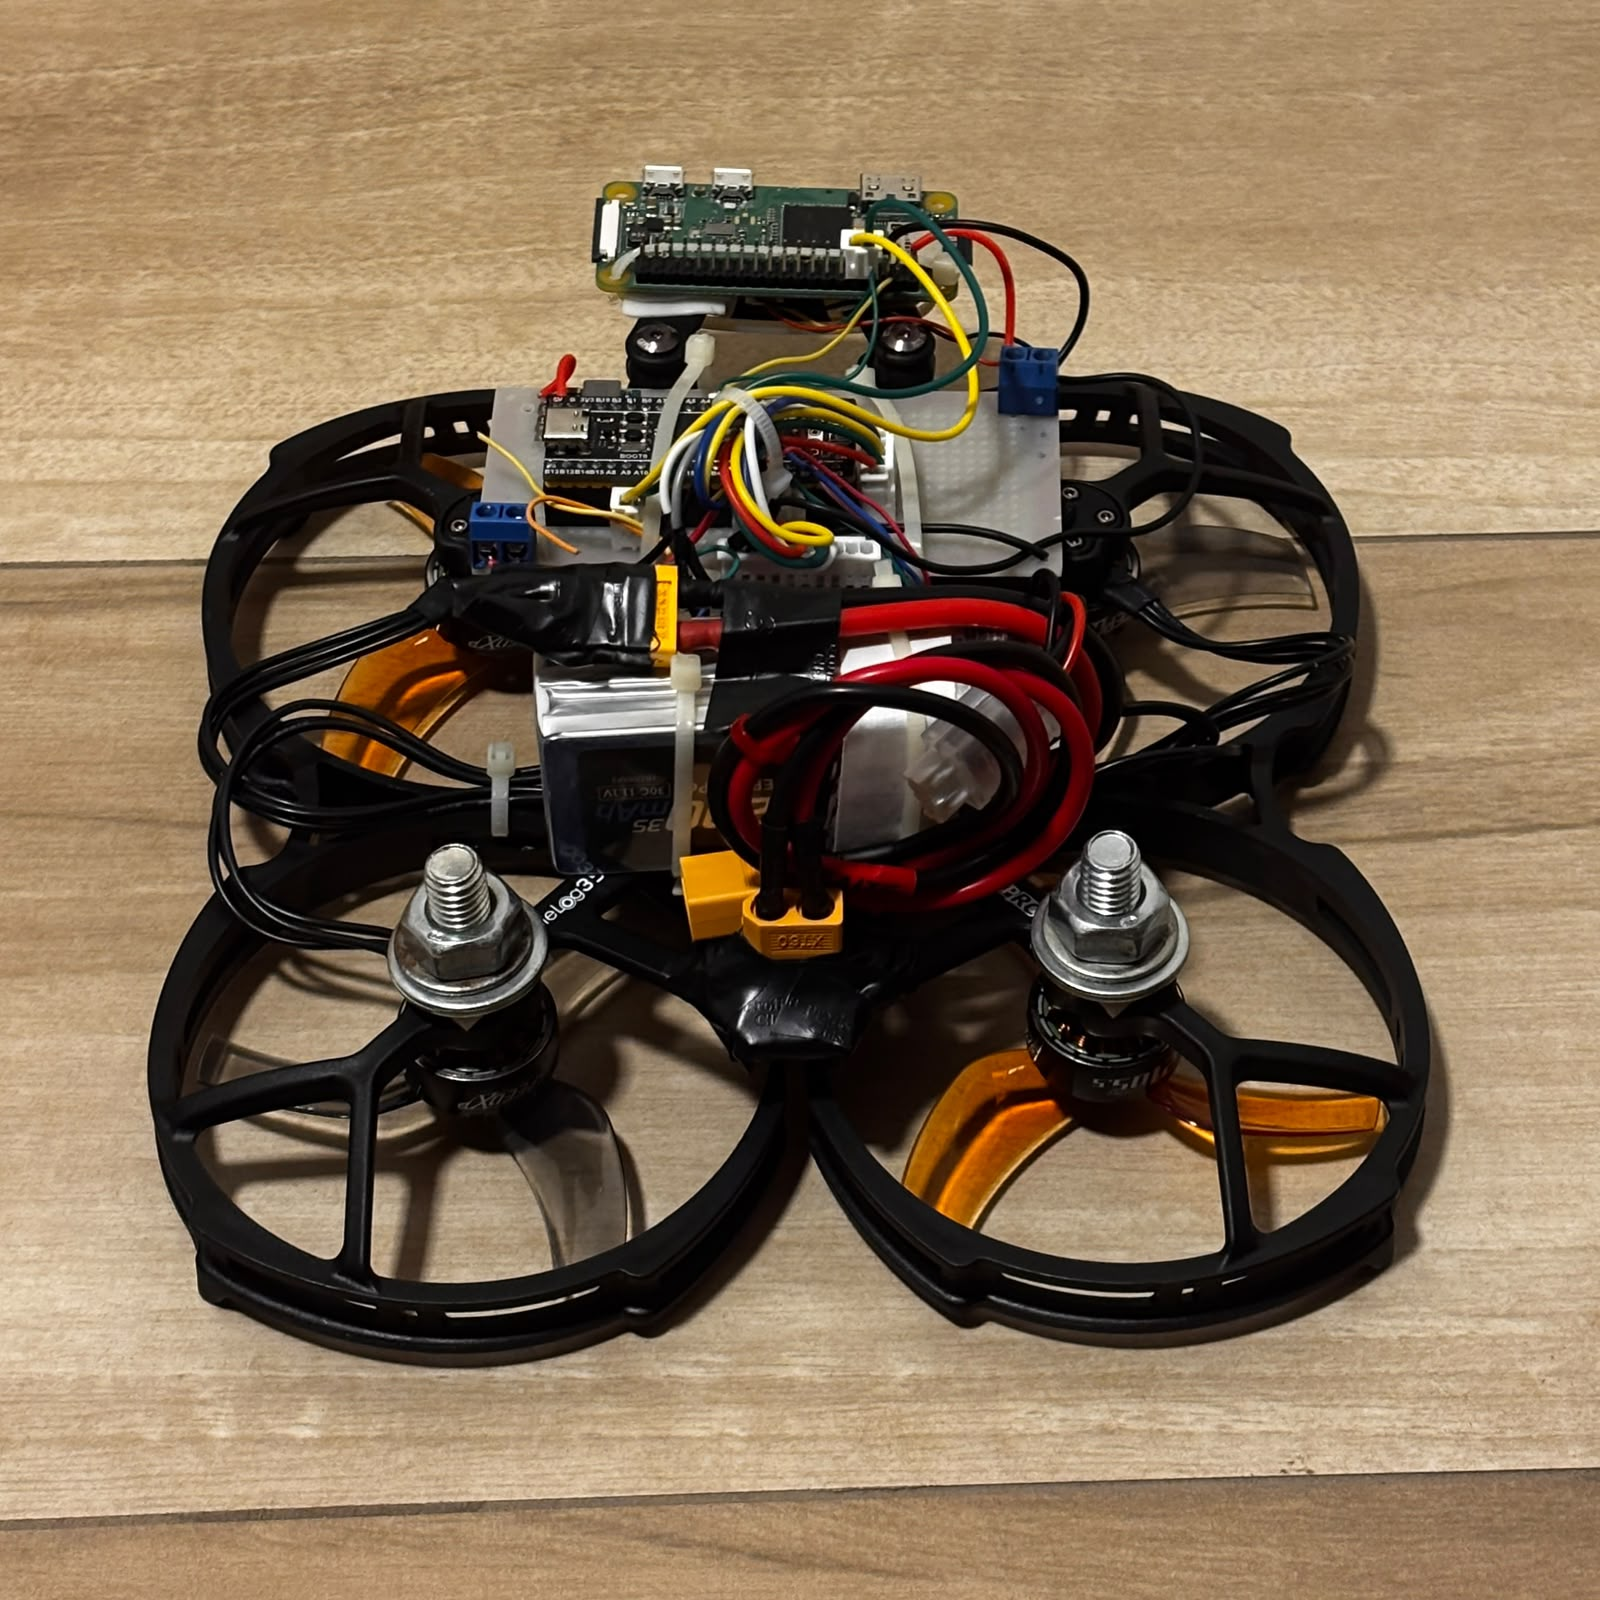
\includegraphics[width=\linewidth,height=4.4cm,keepaspectratio]{images/hardware/prototipo/drone_frente.jpeg}
        \par\smallskip{\footnotesize (a) Vista frontal}
    \end{minipage}
    \hfill
    \begin{minipage}[t]{0.31\textwidth}
        \centering
        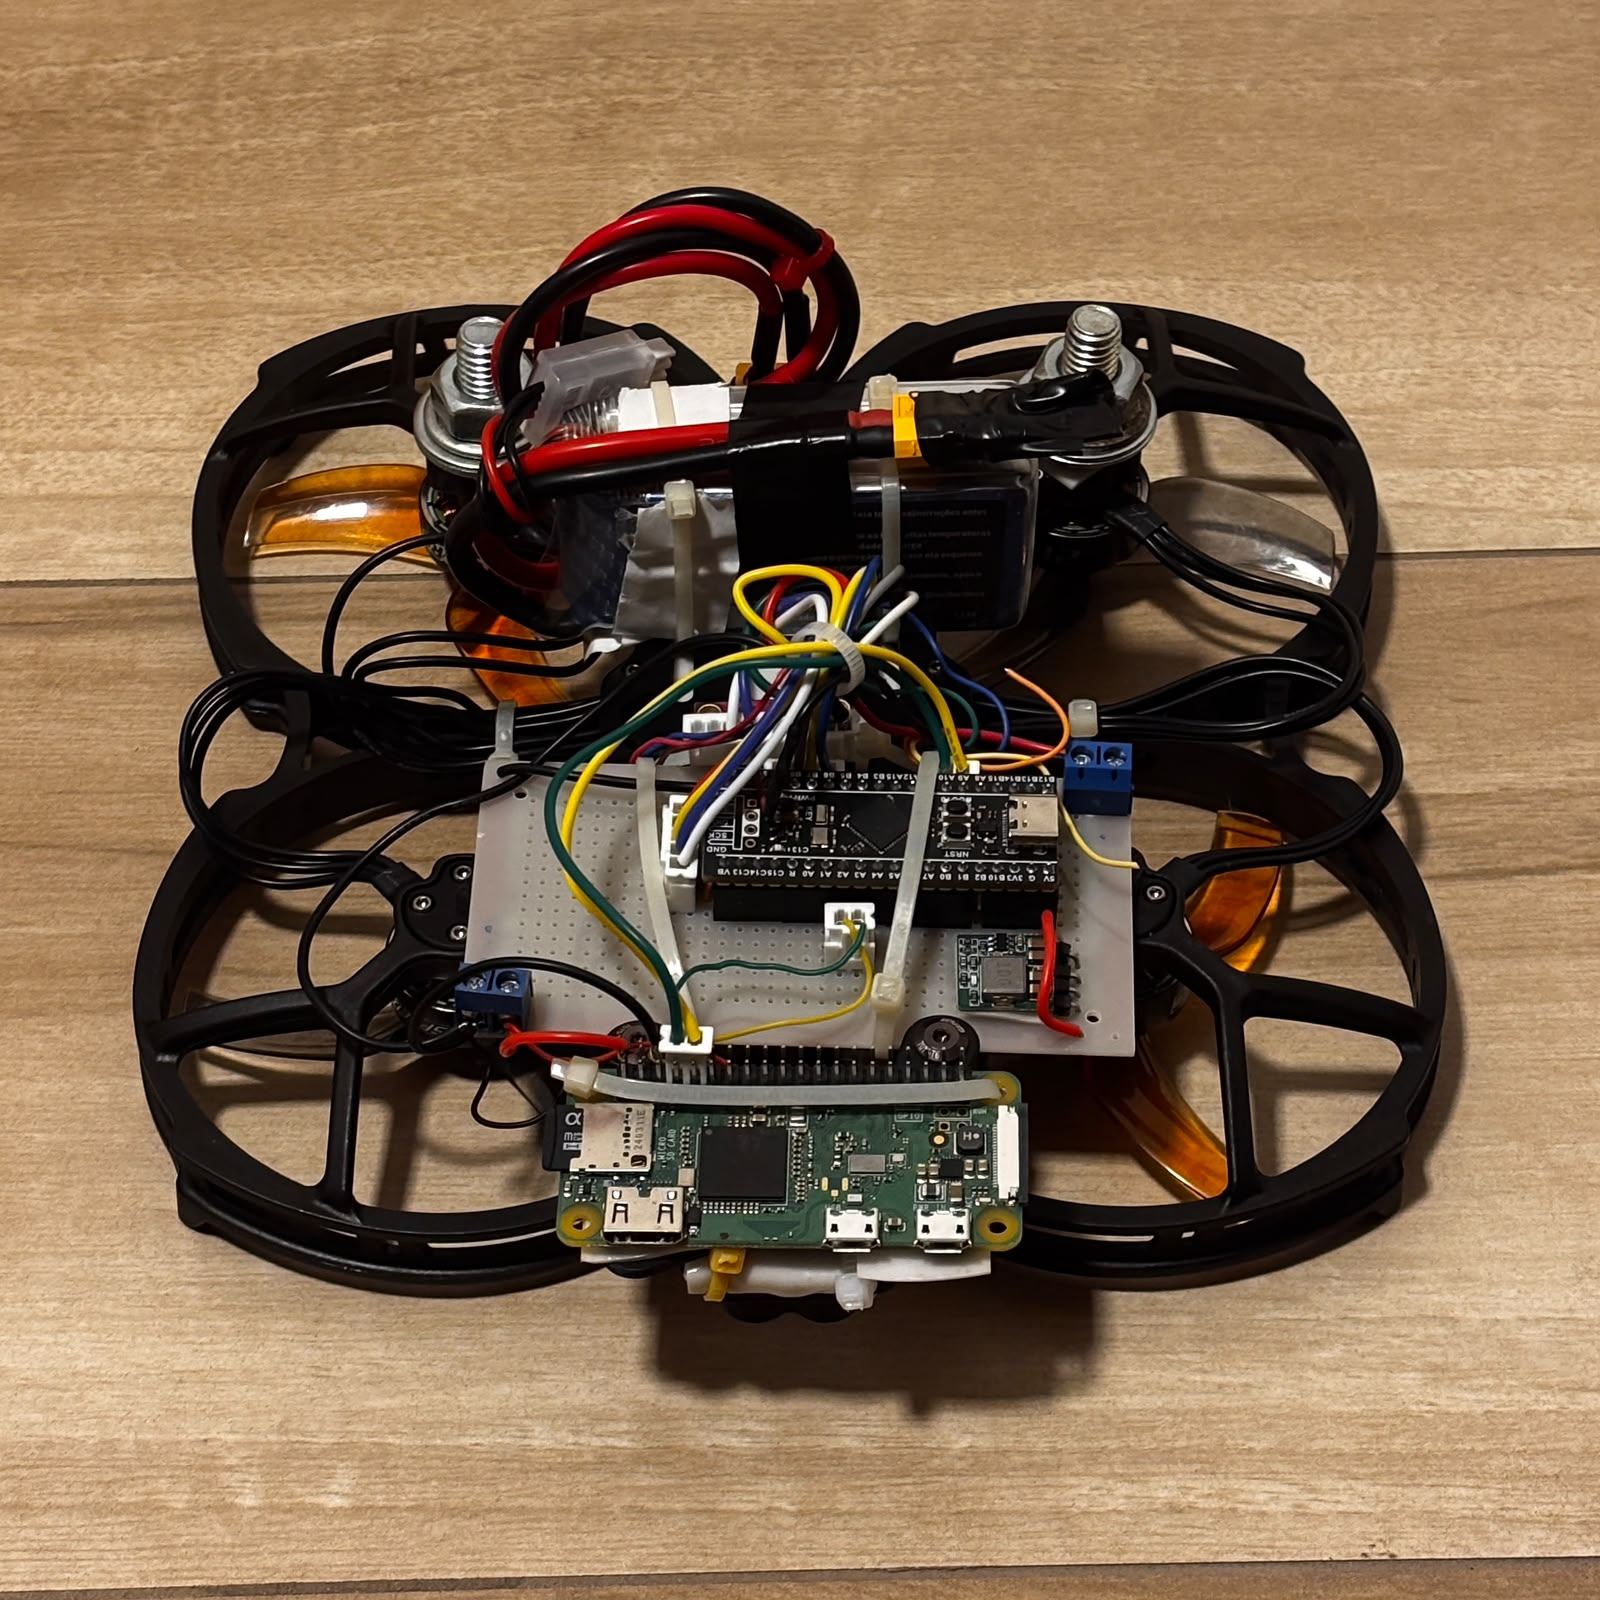
\includegraphics[width=\linewidth,height=4.4cm,keepaspectratio]{images/hardware/prototipo/drone_traseira.jpeg}
        \par\smallskip{\footnotesize (b) Vista traseira}
    \end{minipage}
    \hfill
    \begin{minipage}[t]{0.31\textwidth}
        \centering
        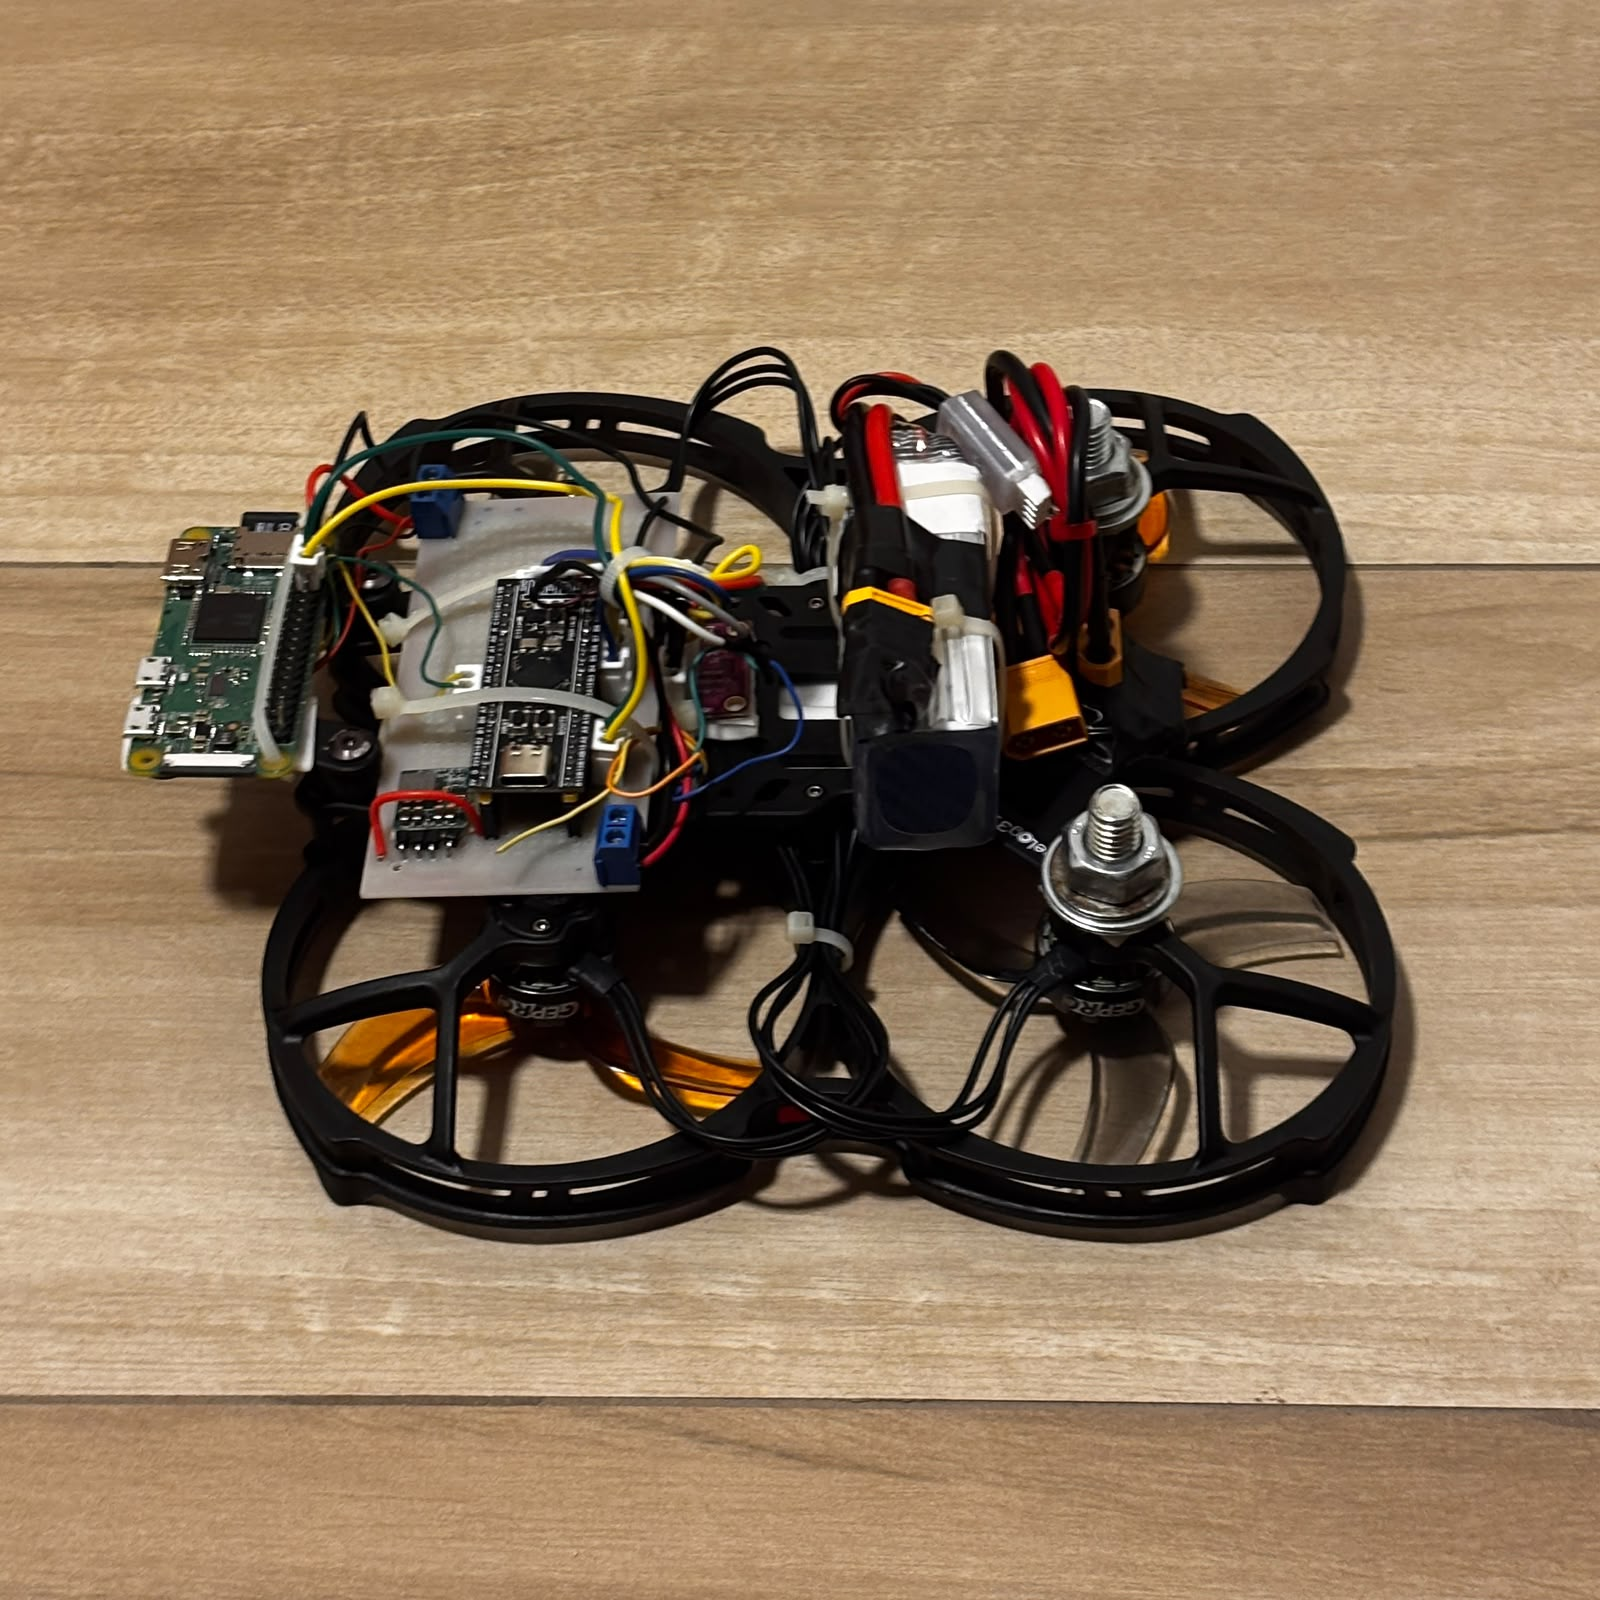
\includegraphics[width=\linewidth,height=4.4cm,keepaspectratio]{images/hardware/prototipo/drone_direita.jpeg}
        \par\smallskip{\footnotesize (c) Lateral direita}
    \end{minipage}
    \par\vspace{0.25cm}
    \begin{minipage}[t]{0.31\textwidth}
        \centering
        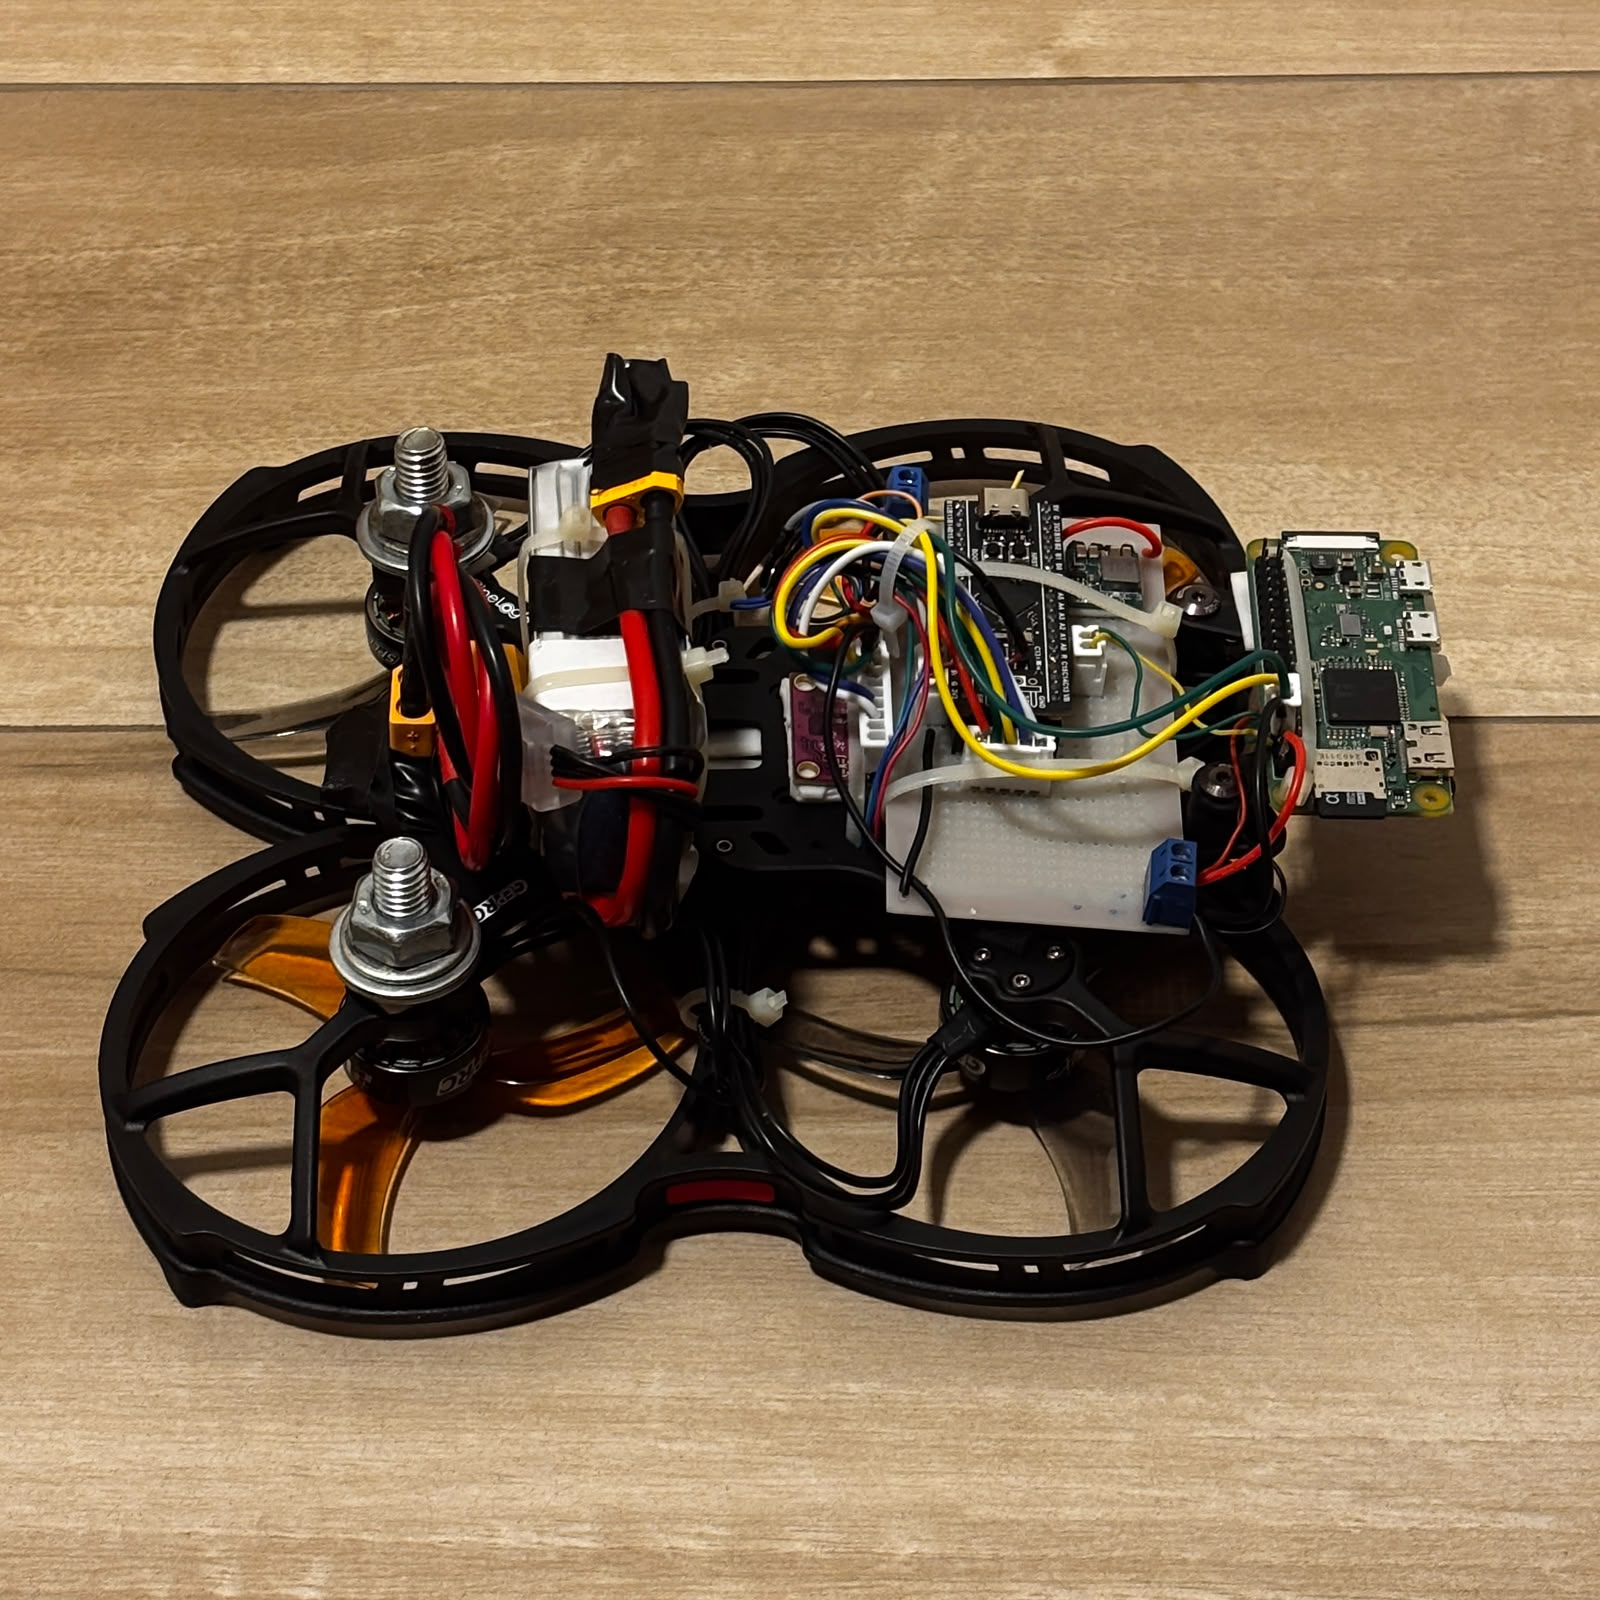
\includegraphics[width=\linewidth,height=4.4cm,keepaspectratio]{images/hardware/prototipo/drone_esquerda.jpeg}
        \par\smallskip{\footnotesize (d) Lateral esquerda}
    \end{minipage}
    \hfill
    \begin{minipage}[t]{0.31\textwidth}
        \centering
        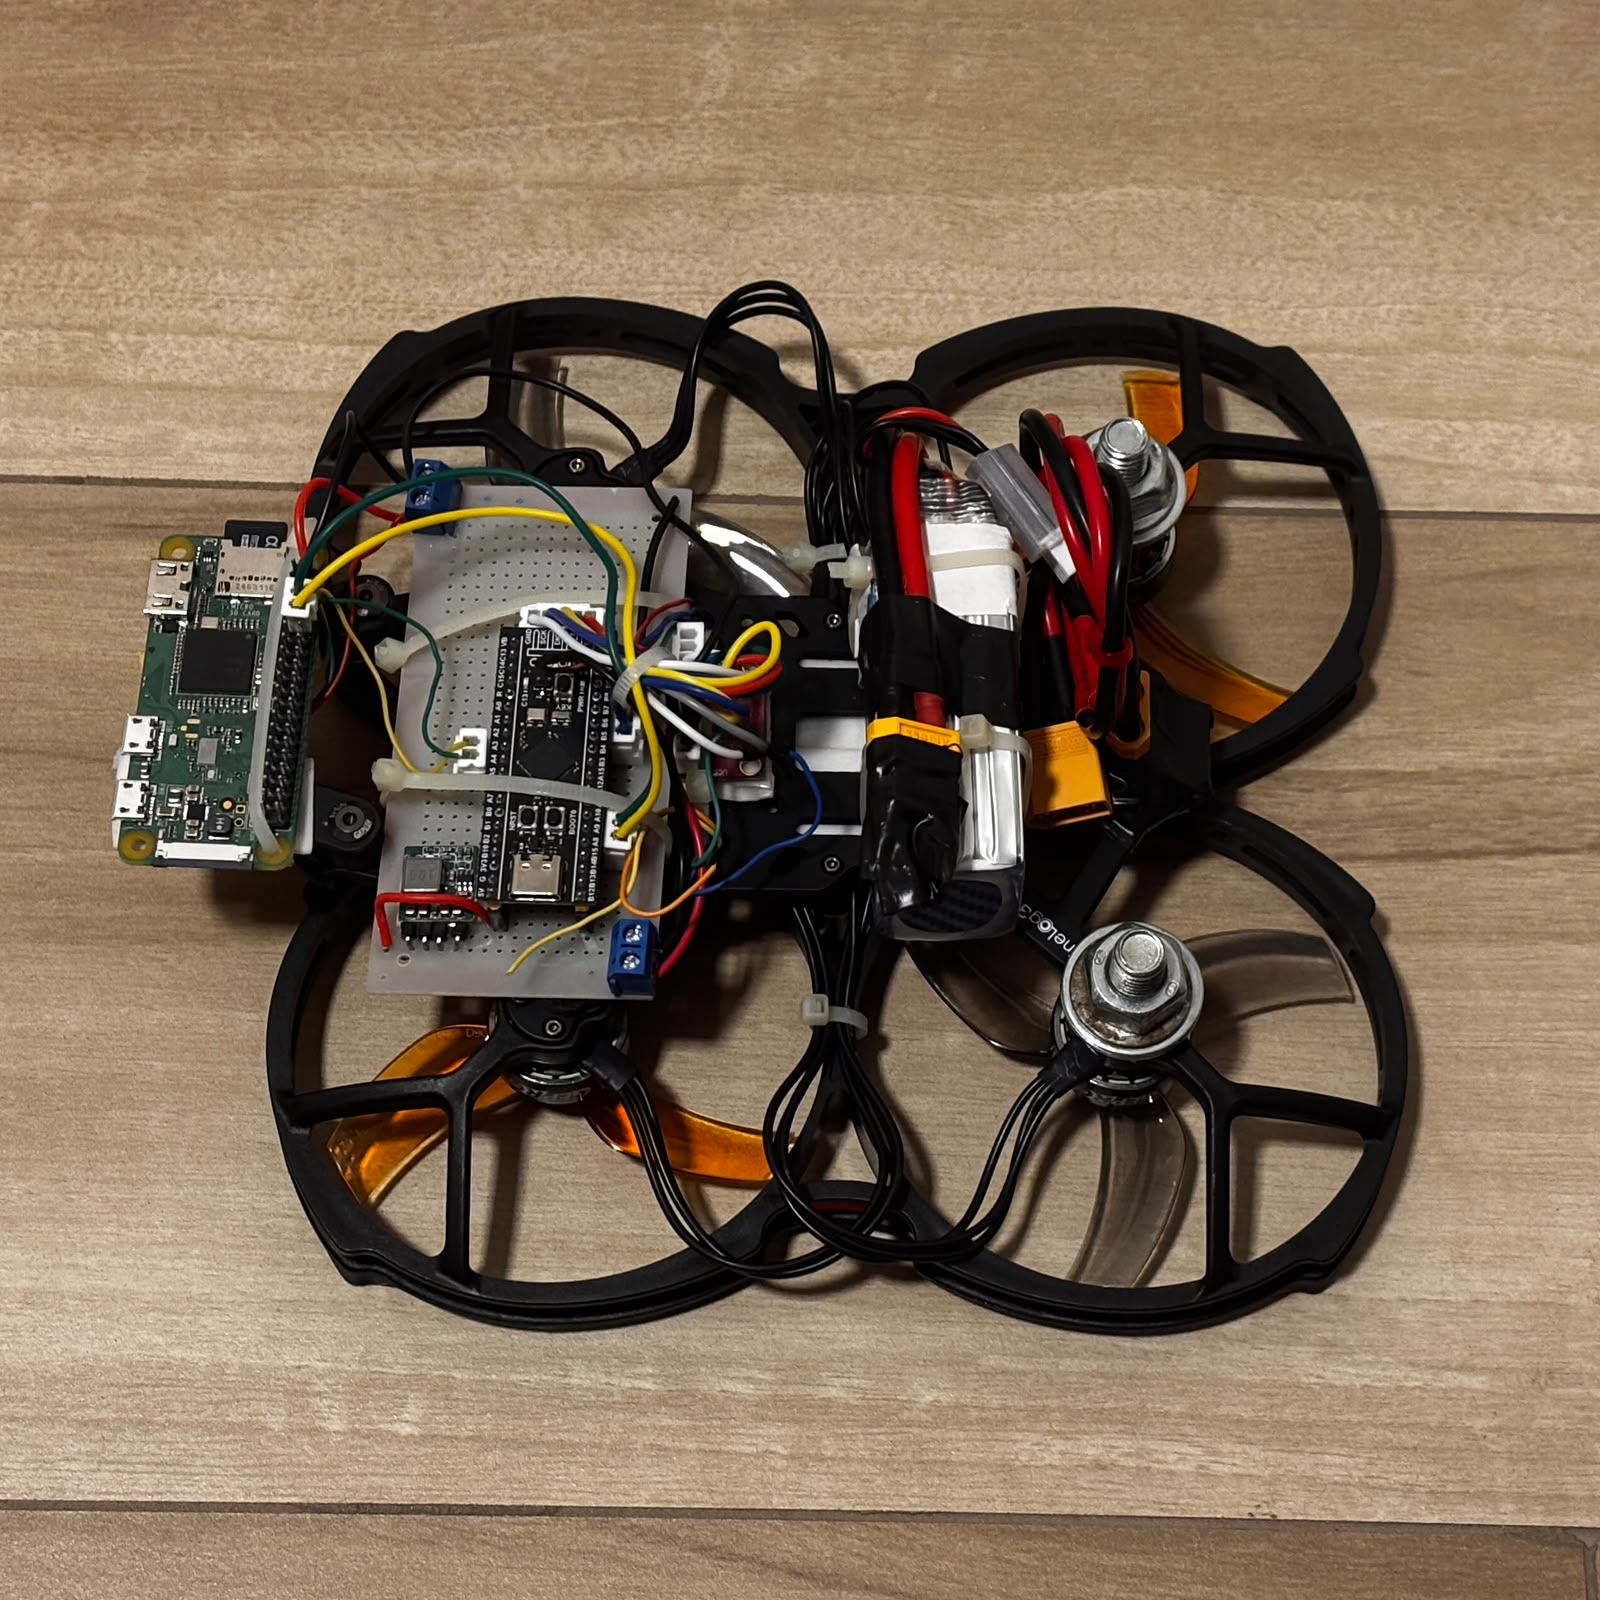
\includegraphics[width=\linewidth,height=4.4cm,keepaspectratio]{images/hardware/prototipo/drone_de_cima.jpeg}
        \par\smallskip{\footnotesize (e) Vista superior}
    \end{minipage}
    \hfill
    \begin{minipage}[t]{0.31\textwidth}
        \centering
        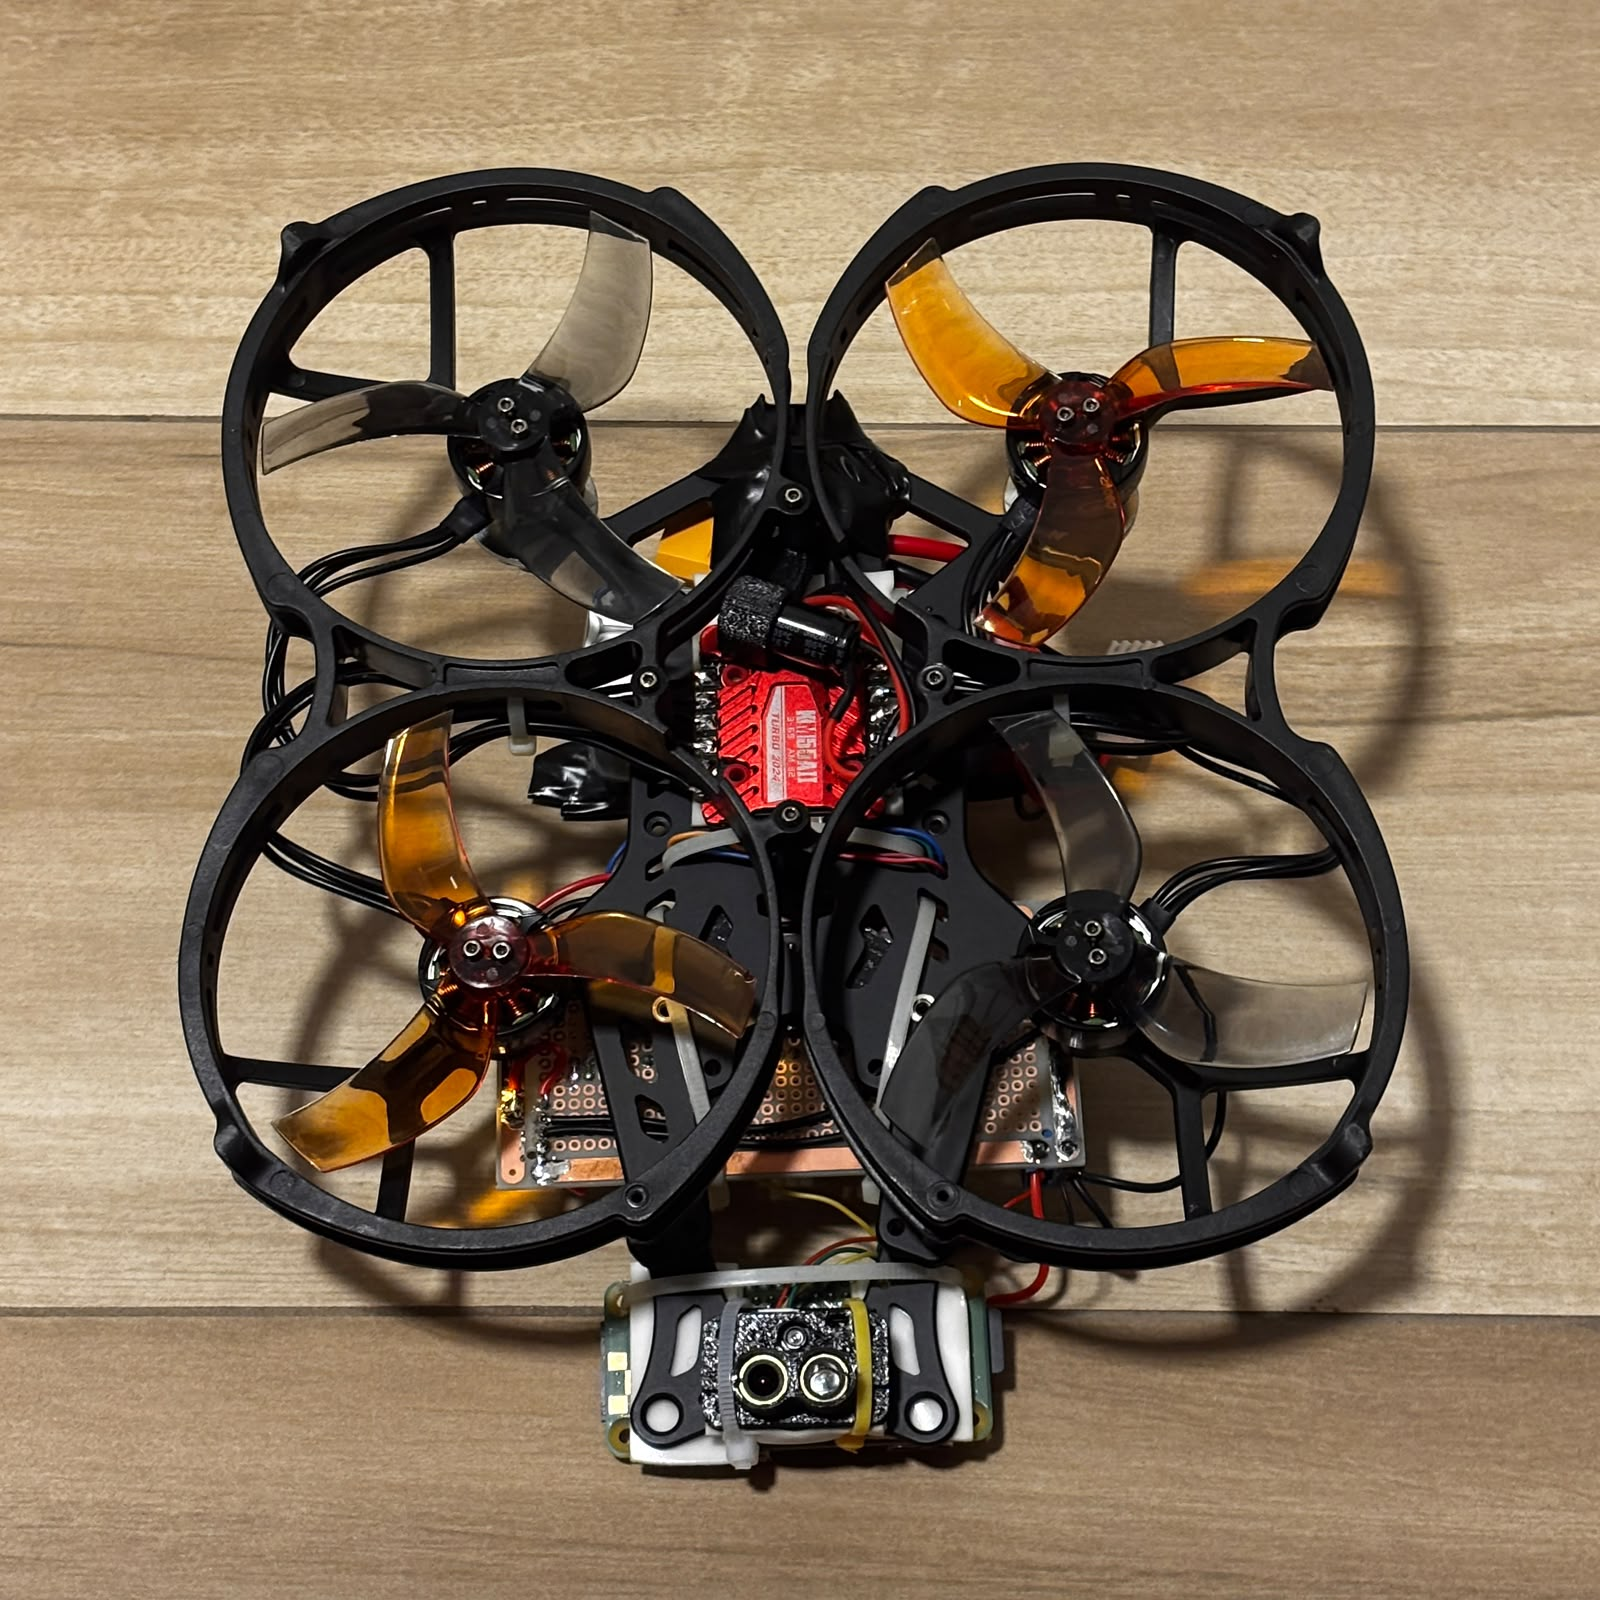
\includegraphics[width=\linewidth,height=4.4cm,keepaspectratio]{images/hardware/prototipo/drone_de_baixo.jpeg}
        \par\smallskip{\footnotesize (f) Vista inferior}
    \end{minipage}
    \par\vspace{0.25cm}
    \footnotesize Fonte: elaborado pelos autores (2026).
\end{figure}

O ambiente de desenvolvimento é apresentado no Quadro~\ref{qua:software}. A versão do projeto e seus arquivos de configuração constituem parte do método, pois permitem reconstruir o ambiente de compilação.

\begin{quadro}[htb]
\centering
\caption{Ambiente de desenvolvimento e versões dos softwares.}
\label{qua:software}
\small
\renewcommand{\arraystretch}{1.3}
\begin{tabular}{
  |
  >{\raggedright\arraybackslash}p{4.5cm}
  |
  >{\raggedright\arraybackslash}p{10.0cm}
  |
}
\hline
\textbf{Elemento} & \textbf{Versão ou configuração} \\
\hline

Sistema Operacional &
Windows 11 Pro 64 bits, versão 10.0.26200, build 26200. \\[4pt]
\hline

STM32CubeIDE &
2.2.0, build 29186\_20260626\_0934 (UTC). \\[4pt]
\hline

STM32CubeMX &
6.18.1-RC2; banco DB.6.0.181 no arquivo \texttt{.ioc} (identificação interna completa preservada). \\[4pt]
\hline

STM32CubeProgrammer &
2.23.0. \\[4pt]
\hline

Compilador &
GNU Tools for STM32 14.3.rel1.20251027-0700\newline
\texttt{arm-none-eabi-gcc} 14.3.1. \\[4pt]
\hline

Bibliotecas STM32 &
STM32CubeF4 1.28.3\newline
HAL 1.8.5\newline
CMSIS Device 2.6.11\newline
CMSIS Core 5.6.0\newline
FreeRTOS 10.3.1 e CMSIS-RTOS2, registradas no projeto \texttt{DroneController}. \\[4pt]
\hline

MATLAB/Simulink &
MATLAB R2024a. \\[4pt]
\hline

Raspberry Pi &
Raspbian GNU/Linux 13 (trixie), Debian 13.4\newline
kernel 6.18.34+rpt-rpi-v6\newline
Python 3.13.5\newline
\texttt{/dev/serial0}$\rightarrow$\texttt{ttyAMA0}\newline
I$^2$C, SPI e UART habilitados. \\[4pt]
\hline

Ambiente Python no Raspberry Pi &
Ambiente virtual em \texttt{\textasciitilde{}/drone-venv}, criado com \texttt{-{}-system-site-packages}\newline
\texttt{pip} 26.2.1\newline
\texttt{pyserial} 3.5\newline
\texttt{pymavlink} 2.4.49\newline
\texttt{fastcrc} 0.3.6\newline
\texttt{lxml} 5.4.0\newline
Validado com abertura de \texttt{/dev/serial0} a 115200 8N1 e empacotamento/leitura de mensagem \textit{HEARTBEAT} MAVLink 2. \\
\hline
\end{tabular}
\par\vspace{0.2cm}
\footnotesize Fonte: elaborado pelos autores (2026), a partir de inspeção do ambiente de desenvolvimento e do projeto \texttt{DroneController} em 06 set. 2026.
\end{quadro}

O projeto STM32 inicializa GPIO, DMA, TIM4, I$^2$C2, USART1, USART2, SPI1 e FreeRTOS por meio de CMSIS-RTOS2. A rastreabilidade do \textit{firmware} é mantida por arquivos \texttt{.ioc}, identificação de versão, instruções de compilação e registros de \textit{build}.

\section{PROCEDIMENTO DE DESENVOLVIMENTO}\label{sec:procedimento_desenvolvimento}

O desenvolvimento é organizado em três frentes complementares: modelagem e simulação do sistema, implementação embarcada com comunicação entre camadas e planejamento de rotas. Essa sequência permite relacionar o modelo matemático, os sinais disponíveis no protótipo e os comandos enviados aos atuadores antes da realização dos ensaios.

\subsection{Modelagem e projeto do controle}\label{subsec:modelagem_projeto_controle}

A modelagem e simulação do sistema consiste em aplicar técnicas de controle partindo do modelo não linear apresentado no Capítulo~\ref{cap_revisao}. Para isso, é necessário parametrizar o sistema, aplicar a linearização em torno do ponto de voo estacionário e projetar o controlador LQG. A validação do modelo é realizada por simulação no MATLAB/Simulink, comparando a resposta do modelo linearizado com a planta não linear e verificando a robustez frente a variações de parâmetros e perturbações. 

\subsubsection{Parametrização do modelo}\label{subsubsec:paremetrizacao_modelo}

Os parâmetros físicos foram obtidos de diferentes formas: alguns foram medidos diretamente, outros foram obtidos e aproximados através de análises de dados e os restantes foram estimados a partir de medições indiretas. A massa do quadricóptero foi medida com uma balança de precisão, enquanto o centro de massa foi determinado por meio de um método de equilíbrio. O momento de inércia foi estimado utilizando o método de decomposição analítica. As características dos motores e hélices foram obtidas através de testes de bancada.

Utilizando uma balança e medindo as dimensões físicas do chassis do drone, foi obtido os seguintes parâmetros do Quadro~\ref{qua:parametros_chassis}.

\begin{quadro}[H]
\centering
\caption{Parâmetros físicos e geométricos do chassi.}
\label{qua:parametros_chassis}
\small
\renewcommand{\arraystretch}{1.3}
\begin{tabular}{
  |
  >{\raggedright\arraybackslash}p{6.8cm}
  |
  >{\centering\arraybackslash}p{2.5cm}
  |
  >{\raggedright\arraybackslash}p{3.5cm}
  |
}
\hline
\textbf{Parâmetro} & \textbf{Variável} & \textbf{Valor} \\
\hline

Massa do corpo central (sem motores) & $M_d$ & 0,463~kg \\[4pt]
\hline

Massa de cada motor & $M_m$ & 0,022~kg \\[4pt]
\hline

Massa total da aeronave & $M$ & 0,551~kg \\[4pt]
\hline

Distância do centro de massa ao motor & $l$ & 0,142~m \\[4pt]
\hline

Comprimento do corpo central & $a$ & 0,104~m \\[4pt]
\hline

Largura do corpo central & $b$ & 0,104~m \\[4pt]
\hline

Altura do corpo central & $c$ & 0,050~m \\[4pt]
\hline

\end{tabular}
\par\vspace{0.2cm}
\footnotesize Fonte: elaborado pelos autores (2026).
\end{quadro}

Para a determinação dos momentos de inércia, empregou-se o método de decomposição analítica proposto por \citeonline{bouabdallah2007}. A decomposição analítica consiste em decompor o quadricóptero em partes, calcular os momentos de inércia de cada parte e somá-los para obter o momento de inércia total. O Quadro~\ref{qua:parametros_inerciais} apresenta os valores obtidos.

\begin{quadro}[H]
\centering
\caption{Parâmetros inerciais do chassi.}
\label{qua:parametros_inerciais}
\small
\renewcommand{\arraystretch}{1.3}
\begin{tabular}{
  |
  >{\raggedright\arraybackslash}p{6.8cm}
  |
  >{\centering\arraybackslash}p{2.5cm}
  |
  >{\raggedright\arraybackslash}p{3.5cm}
  |
}
\hline
\textbf{Parâmetro} & \textbf{Variável} & \textbf{Valor} \\
\hline

Momento de inércia total no eixo x & $I_{xx}$ & 0,00051~kg.m² \\[4pt]
\hline

Momento de inércia total no eixo y & $I_{yy}$ & 0,00051~kg.m² \\[4pt]
\hline

Momento de inércia total no eixo z & $I_{zz}$ & 0,00083~kg.m² \\[4pt]
\hline

\end{tabular}
\par\vspace{0.2cm}
\footnotesize Fonte: elaborado pelos autores (2026).
\end{quadro}

Por fim, os parâmetros aerodinâmicos foram obtidos experimentalmente por meio de ensaios em bancada. A configuração experimental consistiu em uma balança digital invertida, fixada a uma estrutura de suporte e com o prato de pesagem desinstalado, conforme ilustrado na Figura \ref{fig:bancada_teste}. O conjunto propulsor, equipado com os motores GEPRC SPEEDX2 2105.5, também foi montado de forma invertida, procedendo-se com a calibração de tara da balança. O consumo elétrico foi monitorado por meio de um multímetro acoplado a uma fonte de alimentação chaveada. Durante os ensaios, registraram-se o empuxo estático, a corrente consumida e a rotação angular dos motores em função do incremento do comando digital via protocolo DShot.

\begin{figure}[H]
    \centering
    \caption{Bancada de teste de empuxo dos motores.}
    \label{fig:bancada_teste}
    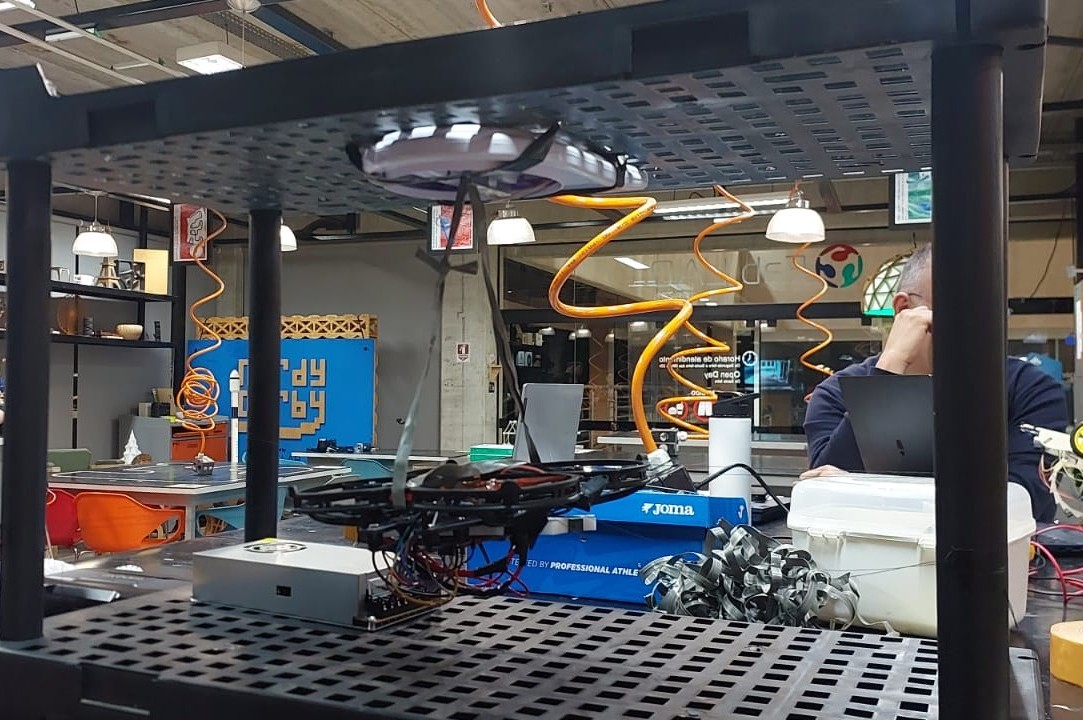
\includegraphics[width=0.85\textwidth]{images/metodologia/bancada_testes.jpeg}
    \par\vspace{0.2cm}
    \footnotesize Fonte: elaborado pelos autores (2026).
\end{figure}

Para determinar as constantes aerodinâmicas a partir dos dados brutos, utilizaram-se abordagens distintas para o empuxo e para o torque. A força de empuxo estático foi modelada pela equação física $T = K_t \omega^2$. Os dados coletados pela balança em gramas-força foram convertidos para Newtons ($1\,\text{gf} \approx 0{,}00981\,\text{N}$) e o coeficiente de empuxo ($K_t$) foi obtido por meio de regressão linear (método dos mínimos quadrados) utilizando a biblioteca \textit{SciPy} em Python, ajustando-se a curva teórica aos pontos experimentais.

Na ausência de um dinamômetro torcional na bancada, o coeficiente de torque ($K_q$) foi estimado de forma indireta por meio do princípio da conservação de potência em máquinas elétricas \cite{chapman2013}. Sabendo que a potência mecânica no eixo do motor é dada por $P_{mec} = \tau \omega$ (com $\tau = K_q \omega^2$) e a potência elétrica ativa consumida é $P_{ele} = V I$, a relação de transferência de energia assume a forma $K_q \omega^3 = \eta V I$, onde $V$ é a tensão da bateria, $I$ a corrente medida e $\eta$ a eficiência eletromecânica do motor \textit{brushless} (BLDC). Como motores de multirrotores operam com perdas aerodinâmicas e térmicas expressivas sob carga \cite{quan2017}, assumiu-se uma eficiência conservadora de $65\%$ ($\eta = 0{,}65$). A partir dessa formulação, calculou-se o valor de $K_q$ ponto a ponto para o regime estabilizado (acima de $100\,\text{rad/s}$) e adotou-se a sua média aritmética.

A Figura \ref{fig:curvas_aerodinamicas} ilustra os pontos coletados experimentalmente e a curva ajustada para o empuxo. Devido a limitações de fornecimento de corrente da fonte chaveada utilizada na bancada, a coleta de dados foi restrita à velocidade angular máxima de aproximadamente $1200\,\text{rad/s}$. A resposta aerodinâmica para rotações superiores é representada por uma linha de tendência, consistindo na extrapolação do modelo quadrático ajustado.

\begin{figure}[H]
\centering
\caption{Curva experimental de empuxo em função da velocidade angular.}
\label{fig:curvas_aerodinamicas}
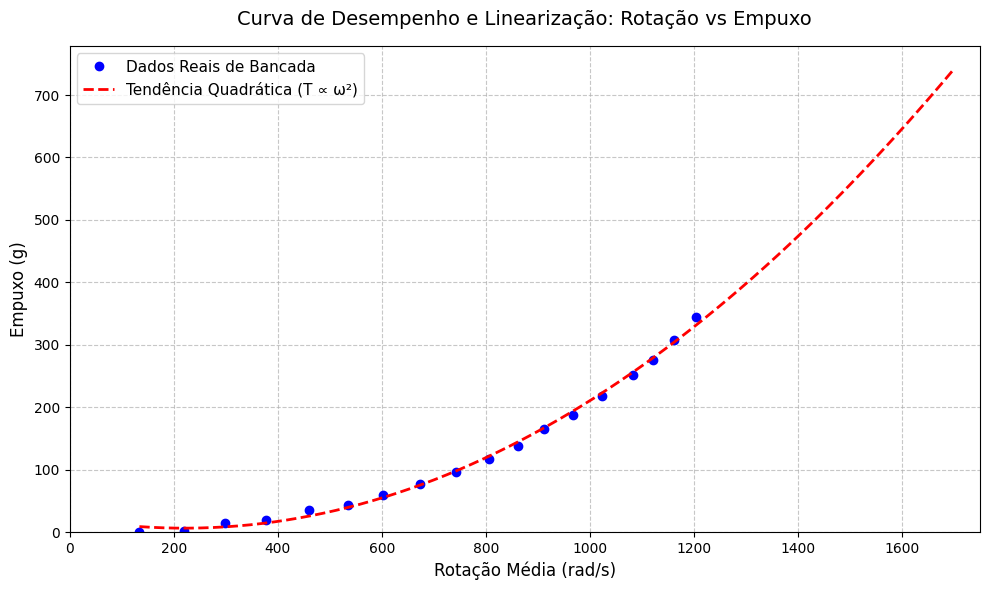
\includegraphics[width=0.75\textwidth]{images/metodologia/empuxo_x_rotacao.png}
\vspace{0.2cm}
\par\footnotesize Fonte: elaborado pelos autores (2026).
\end{figure}

Os valores finais extraídos da regressão, fundamentais para a modelagem dinâmica do sistema no espaço de estados, estão sintetizados no Quadro \ref{qua:parametros_aerodinamicos}.

\begin{quadro}[H]
\centering
\caption{Parâmetros aerodinâmicos das hélices.}
\label{qua:parametros_aerodinamicos}
\small
\renewcommand{\arraystretch}{1.3}
\begin{tabular}{|>{\raggedright\arraybackslash}p{4.8cm}|>{\centering\arraybackslash}p{2.5cm}|>{\centering\arraybackslash}p{5.5cm}|}
\hline
\textbf{Parâmetro} & \textbf{Variável} & \textbf{Valor} \\
\hline
Coeficiente de empuxo & $K_t$ & $2{,}09 \times 10^{-6} \mathrm{\, N\cdot s^2/rad^2}$ \\[4pt]
\hline
Coeficiente de torque & $K_q$ & $2{,}61 \times 10^{-5} \mathrm{\, N\cdot m\cdot s^2/rad^2}$ \\[4pt]
\hline
\end{tabular}
\par\vspace{0.2cm}
\footnotesize Fonte: elaborado pelos autores (2026).
\end{quadro}

\subsubsection{Linearização do sistema}\label{subsubsec:linearizacao_sistema}

Conforme apresentado no Capítulo~\ref{cap_revisao}, a linearização do modelo não linear é realizada em torno do ponto de equilíbrio de voo estacionário (\textit{hover}), onde $\phi_0 = \theta_0 = \psi_0 = 0\text{~rad}$, as velocidades lineares e angulares são nulas e o empuxo total equilibra o peso da aeronave ($T_0 = M g \approx 5{,}4\text{~N}$). Como os quatro conjuntos propulsores dividem igualmente a sustentação no equilíbrio, a velocidade angular nominal de cada rotor é dada por:

\begin{equation}\label{eq:omega_hover}
\omega_0 = \sqrt{\frac{M g}{4 K_t}} = \sqrt{\frac{0,551 \times 9{,}81}{4 \times 2{,}09 \times 10^{-6}}} \approx 804~\text{rad/s}.
\end{equation}

\noindent em que $K_t$ é o coeficiente de empuxo e $K_q$ é o coeficiente de torque aerodinâmico das hélices.

Definindo o vetor de estados $\mathbf{x} \in \mathbb{R}^{12}$ e tomando diretamente as velocidades de rotação dos quatro motores como o vetor de entradas $\mathbf{u} \in \mathbb{R}^{4}$:

\begin{equation}\label{eq:vetores_x_u_motores}
\begin{aligned}
\mathbf{x} &= \begin{bmatrix} x & y & z & \phi & \theta & \psi & \dot{x} & \dot{y} & \dot{z} & p & q & r \end{bmatrix}^T, \\
\mathbf{u} &= \begin{bmatrix} \omega_1 & \omega_2 & \omega_3 & \omega_4 \end{bmatrix}^T,
\end{aligned}
\end{equation}

\noindent aplica-se a expansão em série de Taylor de primeira ordem. A avaliação da matriz Jacobiana de estados $\mathbf{A} = \left.\partial \mathbf{f}/\partial \mathbf{x}\right|_{(\mathbf{x}_0,\mathbf{u}_0)}$ resulta na matriz esparsa $12 \times 12$:

\begin{equation}\label{eq:matriz_A_linear}
\setlength{\arraycolsep}{3.5pt}
\mathbf{A} = 
\begin{bmatrix}
0 & 0 & 0 & 0 & 0 & 0 & 1 & 0 & 0 & 0 & 0 & 0 \\
0 & 0 & 0 & 0 & 0 & 0 & 0 & 1 & 0 & 0 & 0 & 0 \\
0 & 0 & 0 & 0 & 0 & 0 & 0 & 0 & 1 & 0 & 0 & 0 \\
0 & 0 & 0 & 0 & 0 & 0 & 0 & 0 & 0 & 1 & 0 & 0 \\
0 & 0 & 0 & 0 & 0 & 0 & 0 & 0 & 0 & 0 & 1 & 0 \\
0 & 0 & 0 & 0 & 0 & 0 & 0 & 0 & 0 & 0 & 0 & 1 \\
0 & 0 & 0 & 0 & -g & 0 & 0 & 0 & 0 & 0 & 0 & 0 \\
0 & 0 & 0 & g & 0 & 0 & 0 & 0 & 0 & 0 & 0 & 0 \\
0 & 0 & 0 & 0 & 0 & 0 & 0 & 0 & 0 & 0 & 0 & 0 \\
0 & 0 & 0 & 0 & 0 & 0 & 0 & 0 & 0 & 0 & 0 & 0 \\
0 & 0 & 0 & 0 & 0 & 0 & 0 & 0 & 0 & 0 & 0 & 0 \\
0 & 0 & 0 & 0 & 0 & 0 & 0 & 0 & 0 & 0 & 0 & 0
\end{bmatrix}.
\end{equation}

Para a matriz de entrada $\mathbf{B} = \left.\partial \mathbf{f}/\partial \mathbf{u}\right|_{(\mathbf{x}_0,\mathbf{u}_0)}$, considera-se a geometria do chassi em configuração ``X'', na qual os braços formam ângulos de $45^\circ$ com os eixos principais do corpo, resultando em um braço de alavanca efetivo de $l\frac{\sqrt{2}}{2}$ para rolagem e arfagem. Derivando os esforços propulsivos quadráticos ($T_i = K_t\omega_i^2$ e $\tau_{\psi,i} = K_q\omega_i^2$) em torno da rotação de equilíbrio $\omega_0$, obtém-se $\partial T_i/\partial\omega_i = 2K_t\omega_0$, o que conduz à matriz $\mathbf{B} \in \mathbb{R}^{12\times 4}$:

\begin{equation}\label{eq:matriz_B_linear}
\setlength{\arraycolsep}{4pt}
\mathbf{B} = 
\begin{bmatrix}
0 & 0 & 0 & 0 \\
0 & 0 & 0 & 0 \\
0 & 0 & 0 & 0 \\
0 & 0 & 0 & 0 \\
0 & 0 & 0 & 0 \\
0 & 0 & 0 & 0 \\
0 & 0 & 0 & 0 \\
0 & 0 & 0 & 0 \\[2pt]
-\dfrac{2 K_t \omega_0}{M} & -\dfrac{2 K_t \omega_0}{M} & -\dfrac{2 K_t \omega_0}{M} & -\dfrac{2 K_t \omega_0}{M} \\[10pt]
\dfrac{\sqrt{2} l K_t \omega_0}{I_{xx}} & -\dfrac{\sqrt{2} l K_t \omega_0}{I_{xx}} & -\dfrac{\sqrt{2} l K_t \omega_0}{I_{xx}} & \dfrac{\sqrt{2} l K_t \omega_0}{I_{xx}} \\[10pt]
\dfrac{\sqrt{2} l K_t \omega_0}{I_{yy}} & \dfrac{\sqrt{2} l K_t \omega_0}{I_{yy}} & -\dfrac{\sqrt{2} l K_t \omega_0}{I_{yy}} & -\dfrac{\sqrt{2} l K_t \omega_0}{I_{yy}} \\[10pt]
-\dfrac{2 K_q \omega_0}{I_{zz}} & \dfrac{2 K_q \omega_0}{I_{zz}} & -\dfrac{2 K_q \omega_0}{I_{zz}} & \dfrac{2 K_q \omega_0}{I_{zz}}
\end{bmatrix}.
\end{equation}

\subsubsection{Projeto do controlador LQG}\label{subsubsec:projeto_controlador_lqg}

Com o modelo linearizado definido pelas matrizes $\mathbf{A}$ e $\mathbf{B}$, procede-se à síntese do controlador Linear Quadrático Gaussiano (LQG), estruturada em duas etapas independentes conforme o princípio da separação apresentado na Seção~\ref{subsec:lqg}: o cálculo do ganho de realimentação de estados via LQR e o projeto do observador estocástico via Filtro de Kalman.

Para a etapa de regulação (LQR), as matrizes de ponderação de estados $\mathbf{Q} \in \mathbb{R}^{12\times 12}$ e de esforço de controle $\mathbf{R}_{\mathrm{lqr}} \in \mathbb{R}^{4\times 4}$ foram definidas como matrizes diagonais:

\begin{equation}\label{eq:matrizes_Q_R_metodo}
\begin{aligned}
\mathbf{Q} &= \operatorname{diag}\left(q_x,\, q_y,\, q_z,\, q_\phi,\, q_\theta,\, q_\psi,\, q_{\dot{x}},\, q_{\dot{y}},\, q_{\dot{z}},\, q_p,\, q_q,\, q_r\right), \\
\mathbf{R}_{\mathrm{lqr}} &= \operatorname{diag}\left(r_1,\, r_2,\, r_3,\, r_4\right).
\end{aligned}
\end{equation}

Os pesos foram ajustados iterativamente em ambiente de simulação no software MATLAB, priorizando a rápida estabilização das variáveis de atitude ($\phi, \theta, \psi$) e de altitude ($z$), enquanto as ponderações em $\mathbf{R}_{\mathrm{lqr}}$ foram dimensionadas de modo a evitar a saturação prematura dos comandos de velocidade angular enviados aos quatro motores. A partir das matrizes $(\mathbf{A}, \mathbf{B}, \mathbf{Q}, \mathbf{R}_{\mathrm{lqr}})$, obteve-se a matriz de ganho ótimo $\mathbf{K} \in \mathbb{R}^{4\times 12}$.

Na etapa de estimação de estados, a matriz de saída $\mathbf{C}$ foi definida com base nas variáveis efetivamente mensuradas pelo conjunto de sensores da aeronave: a altitude no eixo $z$ e as velocidades lineares nos eixos $x$ e $y$, fornecidas pelo módulo óptico/ToF MTF-01, bem como os ângulos de Euler e as velocidades angulares, obtidos pela unidade de medição inercial BNO08X. Por simplificação de projeto, a matriz de transmissão direta $\mathbf{D}$ foi considerada nula.

A matriz de ruído de processo $\mathbf{Q}_w$ foi ajustada através de simulações, considerando a dinâmica do sistema e a incerteza nos modelos de motores e hélices e a matriz de ruído de medição $\mathbf{R}_v$ foi definida através de testes experimentais, registrando a variância das leituras dos sensores em condições estáticas e em voo:

\begin{equation}\label{eq:matrizes_kalman_metodo}
\mathbf{Q}_w = \operatorname{diag}\left(\sigma_{w,1}^2, \dots, \sigma_{w,12}^2\right), \qquad
\mathbf{R}_v = \operatorname{diag}\left(\sigma_{v,1}^2, \dots, \sigma_{v,p}^2\right).
\end{equation}

Por fim, o acoplamento do estimador com o regulador forma a malha fechada LQG conforme a Figura~\ref{fig:LQRController}. A cada ciclo de controle, o Filtro de Kalman processa as leituras ruidosas $\mathbf{y}$ e a ação de controle anterior para gerar o vetor de estados estimados $\hat{\mathbf{x}}$. O comando total de velocidade angular aplicado aos motores é então calculado somando-se a ação corretiva do LQR à velocidade nominal de equilíbrio $\mathbf{u}_0 = [\omega_0,\, \omega_0,\, \omega_0,\, \omega_0]^{\mathrm{T}}$:

\begin{equation}\label{eq:comando_final_motores}
\mathbf{u} = \mathbf{u}_0 - \mathbf{K}\left(\hat{\mathbf{x}} - \mathbf{x}_{\mathrm{ref}}\right),
\end{equation}

\noindent sendo o vetor resultante $\mathbf{u}$ submetido a um bloco de saturação que restringe as rotações ao intervalo físico operacional dos propulsores $[\omega_{\min},\, \omega_{\max}]$.

\begin{figure}[H]
    \centering
    \caption{Sistema controlador LQG.}
    \label{fig:LQRController}
    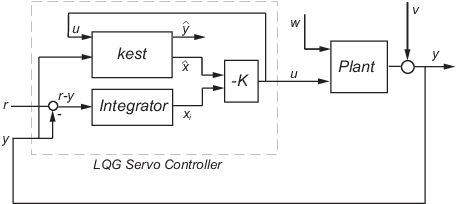
\includegraphics[width=0.8\textwidth]{images/metodologia/LQGController.png}
    \par\vspace{0.2cm}
    \footnotesize Fonte: \citeonline{mathworkslqg}.
\end{figure}

\subsubsection{Comparação entre o sistema linear e o sistema não linear}\label{subsubsec:comp_linear_nao_linear}
Para validar os ganhos obtidos pelo LQR e pelo Filtro de Kalman, foi realizada uma simulação comparativa entre o sistema linearizado e o sistema não linear através do software MATLAB/Simulink. A simulação envolveu a aplicação de perturbações iniciais e a análise da resposta do sistema em termos de estabilidade, tempo de assentamento e overshoot.

\subsection{Implementação embarcada e comunicação}\label{subsec:implementacao_embarcada}

O \textit{firmware} é gerado e compilado com as versões indicadas no Quadro~\ref{qua:software}. FreeRTOS é utilizado para estruturar tarefas e sincronização; consequentemente, o trabalho caracteriza o \textit{firmware} como uma aplicação embarcada com sistema operacional de tempo real. A prioridade e o período de cada tarefa são registrados no código e no relatório de execução.

O barramento I$^2$C2 foi configurado em 400~kHz para a IMU, com PB10 como SCL, PB3 como SDA, PB4 como entrada de interrupção e PB5 como reset. Os canais PB6--PB9 de TIM4 foram reservados para os quatro sinais de motores. A geração DShot por temporizador e DMA é validada primeiro por analisador lógico ou osciloscópio, sem hélices, antes de qualquer ligação aos motores. DShot transmite um valor de \textit{throttle}, um bit de solicitação de telemetria e CRC em uma palavra de 16 bits; o protocolo e seus limites dependem da configuração do ESC \cite{betaflightdshot}.

O ESC utiliza firmware AM32, cuja documentação indica ferramentas de configuração e atualização e suporte ao microcontrolador AT32F421 \cite{am32manual}. Antes de qualquer atualização, os quatro canais são lidos com hélices removidas, registrando-se as versões de \textit{firmware}, \textit{target}, \textit{bootloader} e os parâmetros exportáveis. A identificação da versão instalada é evidência de reprodutibilidade e não pode ser substituída pela versão mais recente disponível na Internet.

% Comunicação Raspberry Pi <-> STM32: enlace, DroneLink, comandos e ensaios
% ============================================================================
% MATERIAIS E MÉTODOS — comunicação entre o Raspberry Pi e o STM32 (DroneLink)
% Chamado em partes/textuais/metodologias.tex, depois de "Implementação
% embarcada e comunicação".
% ============================================================================

\subsection{Comunicação entre o computador de missão e o controlador de voo}\label{subsec:metodo_comunicacao}

A comunicação entre o Raspberry Pi (computador de missão) e o STM32 (controlador de voo) segue o DroneLink, protocolo de aplicação desenvolvido neste trabalho sobre o enquadramento MAVLink 2 (Seção~\ref{subsec:mavlink}). A divisão de responsabilidades é a seguinte: o Raspberry Pi decide \textbf{o que} fazer, isto é, a ordem dos pontos e o próximo objetivo; o STM32 decide \textbf{como} e \textbf{se} fazer, validando cada pedido, executando-o com o controlador LQG e mantendo o VANT seguro mesmo que o Raspberry Pi falhe.

\subsubsection{Enlace físico e ambiente do Raspberry Pi}\label{subsubsec:com_enlace}

No enlace físico entre Raspberry Pi e STM32, a configuração adotada é UART \textit{full-duplex} em lógica de 3,3~V, 115200~bit/s, 8N1 e sem controle de fluxo. O GPIO14/TXD do Raspberry Pi, pino físico 8, liga-se ao PA10/USART1\_RX do STM32; o PA9/USART1\_TX do STM32 liga-se ao GPIO15/RXD do Raspberry Pi, pino físico 10; e o GND comum é obrigatório. No Raspberry Pi, a interface serial está exposta em \texttt{/dev/serial0}, apontando para \texttt{ttyAMA0}, com \texttt{enable\_uart=1}, Bluetooth desabilitado pelo \textit{overlay} \texttt{disable-bt} e console serial desativado, de modo que a UART fique dedicada à comunicação com o controlador de voo.

O software do Raspberry Pi foi desenvolvido em Python 3.13.5, com as bibliotecas \texttt{pyserial} 3.5, \texttt{pymavlink} 2.4.49 e \texttt{numpy} 2.2.4, no Raspberry Pi OS 13 (ARMv6). Sua preparação foi verificada pela abertura da interface serial e pela recepção das mensagens periódicas do STM32. O código e sua organização estão disponíveis no repositório apresentado no Apêndice~\ref{ap:repositorio}.

\subsubsection{Construção do dialeto DroneLink}\label{subsubsec:com_dialeto}

O protocolo é definido em um único arquivo, \texttt{protocol/drone\_controller.xml}, que inclui o \texttt{common.xml} do MAVLink e acrescenta as mensagens próprias do projeto, com identificadores a partir de 51000, faixa não usada pelo \texttt{common.xml}. Desse arquivo são gerados os dois lados do enlace: os \textit{headers} C do STM32, pelo gerador oficial \texttt{mavgen}, e o módulo Python do Raspberry Pi, pela biblioteca \texttt{pymavlink}, que o regera automaticamente sempre que o XML muda. A geração a partir da mesma definição mantém a estrutura das mensagens consistente entre os dois lados, e o \texttt{CRC\_EXTRA} auxilia na detecção de definições incompatíveis.

O STM32 usa o \textit{System ID}~1 e o \textit{Component ID}~1 (piloto automático), e o Raspberry Pi, o mesmo \textit{System ID} com o \textit{Component ID}~191 (computador de bordo). O STM32 só processa mensagens com essa origem e com o destino indicado nos campos \texttt{target\_system} e \texttt{target\_component} de cada mensagem; as demais são ignoradas. As mensagens utilizadas estão no Quadro~\ref{qua:dronelink_mensagens}.

\begin{quadro}[H]
    \centering
    \caption{Mensagens do DroneLink.}
    \label{qua:dronelink_mensagens}
    \footnotesize
    \renewcommand{\arraystretch}{1.25}
    \setlength{\tabcolsep}{3pt}
    \begin{tabular}{|>{\raggedright\arraybackslash}p{4.2cm}|>{\centering\arraybackslash}p{1.1cm}|>{\centering\arraybackslash}p{1.1cm}|>{\raggedright\arraybackslash}p{1.6cm}|>{\raggedright\arraybackslash}p{5.4cm}|}
        \hline
        \textbf{Mensagem} & \textbf{De} & \textbf{Para} & \textbf{Taxa} & \textbf{Função} \\
        \hline
        \multicolumn{5}{|l|}{\textbf{Padrão (\texttt{common.xml})}} \\
        \hline
        \texttt{HEARTBEAT} & Pi & STM32 & 4~Hz & Presença do computador de missão. \\
        \hline
        \texttt{HEARTBEAT} & STM32 & Pi & 2~Hz & Estado de voo e indicação de armado. \\
        \hline
        \texttt{COMMAND\_\allowbreak LONG} & Pi & STM32 & Por pedido & Solicitação de armar ou desarmar. \\
        \hline
        \texttt{COMMAND\_\allowbreak ACK} & STM32 & Pi & Por resposta & Aceite ou recusa do comando. \\
        \hline
        \texttt{PARAM\_\allowbreak *} & Pi & STM32 & Por pedido & Consulta ou alteração de parâmetros. \\
        \hline
        \texttt{PARAM\_\allowbreak VALUE} & STM32 & Pi & Por resposta & Valor efetivamente adotado. \\
        \hline
        \texttt{ATTITUDE, LOCAL\_\allowbreak POSITION\_\allowbreak NED} & STM32 & Pi & 5~Hz & Atitude e posição estimadas. \\
        \hline
        \texttt{SYS\_\allowbreak STATUS, STATUSTEXT} & STM32 & Pi & Periódica / por evento & Estado do sistema e avisos; bateria quando disponível. \\
        \hline
        \texttt{TIMESYNC} & Pi & STM32 & Por pedido & Solicitação de sincronização dos relógios. \\
        \hline
        \texttt{TIMESYNC} & STM32 & Pi & Por resposta & Horário local para sincronização. \\
        \hline
        \multicolumn{5}{|l|}{\textbf{Próprias do DroneLink}} \\
        \hline
        \texttt{DRONE\_\allowbreak PROTOCOL\_\allowbreak INFO} & STM32 & Pi & 1~Hz & Versão, identidade de boot e capacidades. \\
        \hline
        \texttt{DRONE\_\allowbreak LEG\_\allowbreak COMMAND} & Pi & STM32 & Por pedido & Solicitação de um trecho. \\
        \hline
        \texttt{DRONE\_\allowbreak LEG\_\allowbreak ACK} & STM32 & Pi & Por resposta & Situação e resultado do trecho. \\
        \hline
        \texttt{DRONE\_\allowbreak LEG\_\allowbreak CANCEL} & Pi & STM32 & Por pedido & Cancelamento do trecho. \\
        \hline
        \texttt{DRONE\_\allowbreak CONTROL\_\allowbreak LEASE} & Pi & STM32 & 5~Hz & Autorização válida por 1~s. \\
        \hline
        \texttt{DRONE\_\allowbreak GAIN\_\allowbreak ROW, DRONE\_\allowbreak GAIN\_\allowbreak COMMIT} & Pi & STM32 & Por ajuste & Envio e aplicação dos ganhos do LQG. \\
        \hline
        \texttt{DRONE\_\allowbreak GAIN\_\allowbreak ACK} & STM32 & Pi & Por resposta & Resultado do ajuste dos ganhos. \\
        \hline
        \texttt{DRONE\_\allowbreak CTRL\_\allowbreak DEBUG} & STM32 & Pi & Por ajuste & Medições, estimativas, comandos e referências. \\
        \hline
    \end{tabular}
    \par\vspace{0.2cm}
    \footnotesize Fonte: elaborado pelos autores (2026).
\end{quadro}

\subsubsection{Trecho de missão (\textit{leg})}\label{subsubsec:com_trecho}

Um trecho é uma ação solicitada pelo Raspberry Pi ao STM32, como decolar, girar, deslocar-se, manter a posição ou pousar. O pedido contém a ação, o alvo, os limites de execução e os identificadores que o associam à missão e à resposta correspondente.

Antes de aceitar o pedido, o STM32 verifica sua compatibilidade com o estado do veículo, os limites de movimento e as condições de comunicação e autorização. Se o pedido for recusado, o controlador informa o motivo por meio dos códigos apresentados no Quadro~\ref{qua:dronelink_motivos}.

As respostas são enviadas em campos numéricos da mensagem \texttt{DRONE\_LEG\_ACK}, indicando se a operação está em andamento, foi concluída, recusada ou falhou. Os nomes apresentados no quadro correspondem aos identificadores em inglês definidos pelo protocolo.

Na decolagem e nos trechos de movimento, a conclusão depende de o veículo permanecer no alvo por 1~s, dentro das tolerâncias definidas e com velocidades estimadas baixas. Nos ensaios, foram adotadas tolerâncias de 5~cm para posição e 0,05~rad para guinada, além de limites de 5~cm/s para velocidade linear e 0,1~rad/s para velocidade angular. A confirmação de conclusão é enviada após essa verificação.


\begin{quadro}[H]
    \centering
    \caption{Principais motivos de recusa de um trecho.}
    \label{qua:dronelink_motivos}
    \small
    \renewcommand{\arraystretch}{1.25}
    \begin{tabular}{|>{\raggedright\arraybackslash}p{4.8cm}|>{\raggedright\arraybackslash}p{9cm}|}
        \hline
        \textbf{Motivo} & \textbf{Situação} \\
        \hline
        \texttt{BAD\_STATE} &
        O estado do VANT não permite executar a ação solicitada. \\
        \hline
        \texttt{BUSY} &
        Há outra operação em execução. \\
        \hline
        \texttt{OUT\_OF\_BOUNDS} &
        Algum campo do pedido está fora da faixa permitida. \\
        \hline
        \texttt{STALE\_BOOT} &
        A identidade de inicialização informada não corresponde à atual do STM32. \\
        \hline
        \texttt{SEQUENCE\_ERROR} &
        O índice do trecho não corresponde à sequência esperada. \\
        \hline
        \texttt{OPERATOR\_LEASE\_LOST} &
        A autorização do operador não está ativa. \\
        \hline
        \texttt{LINK\_LOST} &
        O \textit{HEARTBEAT} do Raspberry Pi não é recebido há pelo menos 1~s. \\
        \hline
        \texttt{SENSOR\_UNHEALTHY} &
        Uma condição de sensor necessária à operação não foi atendida. \\
        \hline
        \texttt{ID\_COLLISION} &
        Os mesmos identificadores foram usados em pedidos com conteúdos diferentes. \\
        \hline
    \end{tabular}
    \par\vspace{0.2cm}
    \footnotesize Fonte: elaborado pelos autores (2026).
\end{quadro}

\subsubsection{Idempotência e identidade de \textit{boot}}\label{subsubsec:com_idempotencia}

O Raspberry Pi aguarda até 1~s pela primeira resposta de cada trecho e, se ela não chega, reenvia o mesmo pedido, com os mesmos identificadores, até três vezes. Para que o reenvio seja seguro, o STM32 guarda um histórico circular das 32 últimas transações, com os identificadores e um \textit{hash} do conteúdo. Um pedido repetido recebe a mesma resposta já enviada, sem ser executado de novo, o que implementa a semântica de no máximo uma vez (Seção~\ref{subsec:comunicacao_confiavel}); um pedido com os mesmos identificadores e conteúdo diferente é recusado por colisão de identificador.

A cada inicialização, o STM32 incrementa um contador de \textit{boots} gravado em um registro na memória \textit{flash} externa W25Q64, e o valor é publicado como \texttt{boot\_id}. O Raspberry Pi copia esse valor em todos os pedidos. Se o STM32 reiniciar durante uma missão, os pedidos antigos passam a ser recusados por \textit{boot} desatualizado, impedindo que um comando anterior à reinicialização seja executado. Sem um \texttt{boot\_id} persistente, o STM32 não aceita armar nem executar trechos.

\subsubsection{Supervisão do enlace e da autorização do operador}\label{subsubsec:com_supervisao}

Durante o voo, o STM32 supervisiona o enlace com o Raspberry Pi e a autorização do operador. Em caso de perda, solicita as ações do Quadro~\ref{qua:dronelink_failsafe}: \textit{HOLD}, para manter a posição, ou \textit{LAND}, para pousar.
  

\begin{quadro}[H]
    \centering
    \caption{Ações do STM32 diante da perda do enlace ou da autorização.}
    \label{qua:dronelink_failsafe}
    \small
    \renewcommand{\arraystretch}{1.25}
    \begin{tabular}{|>{\raggedright\arraybackslash}p{7.6cm}|>{\raggedright\arraybackslash}p{6.2cm}|}
        \hline
        \textbf{Condição} & \textbf{Ação solicitada} \\
        \hline
        Sem \textit{HEARTBEAT} do Raspberry Pi por 1~s &
        \textit{Request HOLD}; novos trechos são recusados. \\
        \hline
        Sem \textit{HEARTBEAT} por 2~s e com navegação degradada
        (posição, altura ou atitude inválidas) &
        \textit{Request LAND}. \\
        \hline
        Sem \textit{HEARTBEAT} por 5~s &
        \textit{Request LAND}. \\
        \hline
        Autorização do operador expirada ou retirada &
        \textit{Request HOLD}. \\
        \hline
        Autorização expirada ou retirada por 5~s &
        \textit{Request LAND}. \\
        \hline
    \end{tabular}
    \par\vspace{0.2cm}
    \footnotesize Fonte: elaborado pelos autores (2026), a partir da configuração do protocolo.
\end{quadro}

Essa supervisão vale somente para voos iniciados pelo Raspberry Pi. Voos de bancada comandados pelo console USB do STM32 não dependem do enlace, o que permitiu os ensaios descritos na Seção~\ref{subsubsec:com_ensaios}.

\subsubsection{Implementação no STM32}\label{subsubsec:com_firmware}

No STM32, a comunicação é dividida entre transporte, tratamento do protocolo e telemetria. A USART1 recebe por DMA circular de 512~bytes, e uma tarefa do FreeRTOS processa as mensagens. Na transmissão, respostas de comandos e \textit{HEARTBEAT} têm prioridade sobre a telemetria ainda na fila. Todos os módulos compartilham o contador de sequência MAVLink, necessário à identificação de mensagens ausentes.

O protocolo utiliza o histórico de pedidos e a identidade de inicialização descritos anteriormente. Uma interface de comandos conecta a comunicação ao controle de voo, permitindo que tanto o Raspberry Pi quanto o console USB solicitem ações ao mesmo controlador. A telemetria informa atitude, posição e estado de voo; a altura publicada é medida a partir do chão registrado ao armar, referência também usada na decolagem.

\subsubsection{Ferramenta do Raspberry Pi e comandos do operador}\label{subsubsec:com_comandos}

O programa \texttt{dronectl} permite ao operador executar comandos e missões pelo Raspberry Pi. No modo \texttt{missao}, as instruções podem ser fornecidas pelo terminal ou por arquivo, conforme o Quadro~\ref{qua:dronelink_comandos}.

Por exemplo, durante uma rota, o Raspberry Pi aguarda a confirmação do STM32 antes de avançar ao próximo trecho. Enquanto o trecho está em execução, o controlador informa \texttt{MAV\_RESULT\_IN\_PROGRESS}; ao concluí-lo, envia \texttt{MAV\_RESULT\_ACCEPTED} com progresso de 100\%. Em caso de erro no arquivo ou interrupção pelo operador, o Raspberry Pi solicita o pouso.



\begin{quadro}[H]
    \centering
    \caption{Comandos do operador no modo de missão.}
    \label{qua:dronelink_comandos}
    \footnotesize
    \renewcommand{\arraystretch}{1.25}
    \begin{tabular}{|>{\raggedright\arraybackslash}p{3.6cm}|>{\raggedright\arraybackslash}p{6.2cm}|>{\raggedright\arraybackslash}p{4.1cm}|}
        \hline
        \textbf{Comando} & \textbf{Função} & \textbf{Mensagens enviadas} \\
        \hline
        \texttt{takeoff <cm>} & Arma e sobe até a altura; termina com o VANT estável. & \texttt{COMMAND\_LONG} (armar) e trecho de decolagem \\
        \hline
        \texttt{yaw <graus>} & Gira no lugar; positivo é horário visto de cima. & Trecho de giro \\
        \hline
        \texttt{forward}, \texttt{back}, \texttt{right}, \texttt{left}, \texttt{climb}, \texttt{descend} \texttt{<cm>} & Desloca-se no referencial do corpo. & Trecho de translação \\
        \hline
        \texttt{goto <x> <y> [z]} & Vai ao ponto do referencial local: gira até ficar de frente para ele e anda em linha reta. & Giro, quando necessário, e translação \\
        \hline
        \texttt{waypoints <x,y[,z]> ...} & Executa \texttt{goto} para cada ponto, na ordem dada. & Até dois trechos por ponto \\
        \hline
        \texttt{route [alg] [x,y[,z] ...]} & Executa a rota: ordena os pontos pelo algoritmo escolhido (genético por padrão), visita todos e volta à partida; sem pontos, lê o arquivo de pontos do Raspberry Pi (Seção~\ref{subsubsec:rotas_formulacao_adotada}). & Até dois trechos por ponto \\
        \hline
        \texttt{rtl} & Retorna ao ponto de decolagem (\textit{return to launch}). & Trecho de giro e de translação \\
        \hline
        \texttt{hold} & Mantém a posição atual. & Trecho de HOLD \\
        \hline
        \texttt{land} & Pousa e desarma. & Trecho de pouso \\
        \hline
        \texttt{wait <s>}, \texttt{status}, \texttt{help}, \texttt{exit} & Espera, mostra estado e posição, lista os comandos, encerra (pousando antes, se em voo). & --- \\
        \hline
    \end{tabular}
    \par\vspace{0.2cm}
    \footnotesize Fonte: elaborado pelos autores (2026).
\end{quadro}

Uma missão pode reunir decolagem, execução da rota e pouso, por meio dos comandos \texttt{takeoff}, \texttt{route} e \texttt{land}. No ensaio integrado com o VANT simulado, foram escolhidos três pontos que, junto ao ponto de partida, formam um quadrado de 40~cm de lado. Esse percurso simples permitiu verificar a visita aos pontos e o retorno à origem; trata-se de um cenário de teste, e não de uma restrição do planejamento de rotas.

\subsubsection{Procedimento de ensaio}\label{subsubsec:com_ensaios}

A comunicação foi avaliada por testes automatizados do software do Raspberry Pi, ensaios do STM32 pela USB e um ensaio integrado entre os dois dispositivos pela UART. Os testes verificaram a troca de mensagens, a sequência de comandos, as recusas e as respostas a falhas.

Nos ensaios com o STM32, utilizou-se o modo \texttt{FLT\_SIM = 1}, com os motores desligados. Nesse modo, um modelo linear do veículo, empregado no projeto do controlador LQG e executado no STM32, fornece medições simuladas ao controlador. O modelo também inclui uma representação simplificada do contato com o solo.

A cada ciclo de controle, o modelo calcula a evolução do veículo a partir dos comandos recebidos. A conclusão de um movimento é informada quando o estado simulado atende aos critérios de chegada e estabilidade. Dessa forma, o ensaio avalia a integração entre comunicação e controle, sem reproduzir todas as condições de um voo real.

No ensaio integrado, foram medidas as perdas e os erros de comunicação durante 60~s e a latência de 100 pedidos. Também foram executadas uma missão e verificações de pedidos inválidos ou repetidos, além de interrupções da autorização e do enlace.

Os resultados de comunicação são apresentados na Seção~\ref{subsec:res_com_missao}, separadamente dos ensaios de voo físico da Seção~\ref{sec:resultados_voo}.


% Planejamento de rotas: formulação, algoritmos, AG, benchmark e viabilidade dos exatos
% ============================================================================
% MATERIAIS E MÉTODOS — planejamento de rotas (ordem de visita dos pontos)
% Chamado em partes/textuais/metodologias.tex.
% ============================================================================

\subsection{Planejamento de rotas}\label{subsec:metodo_rotas}

O problema de roteamento é modelado como uma variante do Problema do Caixeiro Viajante para um único VANT (Seção~\ref{subsec:tsp}), no qual cada cromossomo do Algoritmo Genético representa uma ordem válida de visita aos pontos. Como o AG não garante o ótimo global, seu resultado é comparado, sempre sobre o mesmo conjunto de pontos e com sementes registradas, à ordem aleatória, à heurística gulosa e, enquanto viáveis, a dois métodos exatos (Seção~\ref{subsec:rotas_referencias}).

\subsubsection{Formulação adotada}\label{subsubsec:rotas_formulacao_adotada}

O planejamento e a execução da rota são realizados pelo computador de missão. No Raspberry Pi, o operador utiliza o comando \texttt{route} do programa \texttt{dronectl} para informar os pontos a visitar. Os pontos são expressos em centímetros no referencial local, com origem no ponto de decolagem.

Com o VANT em voo e no estado \texttt{HOLD}, o programa calcula a ordem de visita pelo algoritmo genético e envia as ações ao STM32. Para alcançar cada ponto, o veículo gira em sua direção, quando necessário, e se desloca até o alvo, podendo variar a altura durante o movimento. O próximo trecho é enviado após a confirmação de conclusão do anterior. Ao final, o VANT retorna ao ponto de partida, onde o pouso pode ser comandado.

A rota parte de $P_0 = (0, 0, h_0)$, em que $h_0$ é a altura registrada no início da rota, visita todos os pontos e retorna a $P_0$. Seu custo é o comprimento do circuito em três dimensões, conforme as Equações~\ref{eq:rotas_custo} e \ref{eq:rotas_distancia}. As coordenadas fornecidas pelo operador são convertidas de centímetros para metros antes do envio ao STM32.

A função de custo considera apenas a distância percorrida; prazos, tempos de serviço, consumo de energia e obstáculos não são modelados. Assim, a distância é usada como critério simplificado de planejamento, sem garantir o menor tempo de voo ou consumo de energia.

\subsubsection{Algoritmos implementados}\label{subsubsec:rotas_algoritmos}

Os algoritmos do Quadro~\ref{qua:rotas_algoritmos} foram implementados em Python, sem bibliotecas numéricas externas, para que o mesmo código rode no computador pessoal e no Raspberry Pi Zero W. Entre os métodos comparados, apenas a força bruta e o Held-Karp garantem o ótimo global quando concluem o cálculo. Os demais não oferecem essa garantia.

\begin{quadro}[H]
    \centering
    \caption{Algoritmos de ordem de visita comparados.}
    \label{qua:rotas_algoritmos}
    \small
    \renewcommand{\arraystretch}{1.3}
    \begin{tabular}{|>{\raggedright\arraybackslash}p{3.0cm}|>{\centering\arraybackslash}p{2.5cm}|>{\raggedright\arraybackslash}p{8.0cm}|}
        \hline
        \textbf{Algoritmo} & \textbf{Custo} & \textbf{Descrição} \\
        \hline
        Aleatório & $O(N)$ & Uma permutação sorteada; referência do que se obtém sem algoritmo. \\
        \hline
        Guloso & $O(N^2)$ & Vizinho mais próximo a partir de $P_0$; empate resolvido pelo menor índice. \\
        \hline
        Algoritmo genético & $O(G \cdot P \cdot N)$ & $G$ gerações de uma população de $P$ rotas; parâmetros no Quadro~\ref{qua:rotas_parametros_ag}. \\
        \hline
        Força bruta & $O(N \cdot N!)$ & Avalia as $N!$ permutações, sem explorar simetrias. \\
        \hline
        Held-Karp & $O(N^2 2^N)$ & Programação dinâmica sobre subconjuntos; cada estado ocupa 9 \textit{bytes} (custo e predecessor). \\
        \hline
    \end{tabular}
    \par\vspace{0.2cm}
    \footnotesize Fonte: elaborado pelos autores (2026).
\end{quadro}

O algoritmo genético segue a estrutura da Figura~\ref{fig:fluxograma_ag}, sem busca local: a melhora das rotas resulta apenas de seleção, cruzamento e mutação. Seus parâmetros, fixos em todos os ensaios, estão no Quadro~\ref{qua:rotas_parametros_ag}.

\begin{quadro}[H]
    \centering
    \caption{Parâmetros do algoritmo genético.}
    \label{qua:rotas_parametros_ag}
    \small
    \renewcommand{\arraystretch}{1.3}
    \begin{tabular}{|>{\raggedright\arraybackslash}p{3.6cm}|>{\raggedright\arraybackslash}p{10.0cm}|}
        \hline
        \textbf{Elemento} & \textbf{Escolha} \\
        \hline
        Indivíduo & Permutação dos $N$ pontos; $P_0$ fixo no início e no fim. \\
        \hline
        Aptidão & Comprimento do circuito (Equação~\ref{eq:rotas_custo}); menor é melhor. \\
        \hline
        População inicial & 120 permutações aleatórias. \\
        \hline
        Seleção & Torneio de 3 indivíduos; vence o de menor custo. \\
        \hline
        Cruzamento & \textit{Order crossover} (OX) com probabilidade 0,9. \\
        \hline
        Mutação & Inversão de um trecho sorteado, com probabilidade 0,3. \\
        \hline
        Elitismo & Os 2 melhores indivíduos passam diretamente à geração seguinte. \\
        \hline
        Parada & 800 gerações ou 200 gerações consecutivas sem melhora do melhor indivíduo. \\
        \hline
        Semente & 2026, fixa (mesma rota em qualquer máquina). \\
        \hline
    \end{tabular}
    \par\vspace{0.2cm}
    \footnotesize Fonte: elaborado pelos autores (2026).
\end{quadro}

De forma exploratória, avaliou-se também a busca local 2-opt repetida a partir de 20 rotas aleatórias, retendo o melhor ótimo local obtido. Ela não faz parte do comparativo principal e seus resultados são apresentados à parte (Seção~\ref{subsec:res_rotas_2opt}).

\subsubsection{Preparação da comparação dos algoritmos}\label{subsubsec:rotas_benchmark}

Para comparar os algoritmos, foram gerados conjuntos de pontos tridimensionais a serem visitados pelo drone. Cada conjunto representa um cenário de teste, denominado instância. Foram usados de 3 a 30 pontos, com 10 conjuntos diferentes para cada quantidade, totalizando 280 cenários. Os pontos foram sorteados por um programa em Python, usando sementes registradas, isto é, valores que permitem repetir o mesmo sorteio.

Em cada cenário, todos os algoritmos receberam os mesmos pontos e o mesmo local de partida. Foram registrados o comprimento da rota, a ordem de visita e o tempo de cálculo. A Tabela~\ref{tab:rotas_protocolo} resume as condições dessa comparação, também chamada de \textit{benchmark}.

\begin{table}[H]
    \centering
    \caption{Condições da comparação dos algoritmos de rotas.}
    \label{tab:rotas_protocolo}
    \small
    \renewcommand{\arraystretch}{1.25}
    \begin{tabular}{p{4.2cm}p{9.6cm}}
        \hline
        \textbf{Item} & \textbf{Valor} \\
        \hline
        Número de pontos ($N$) & 3 a 30, além de $P_0$ \\
        Cenários por quantidade de pontos & 10 (sementes 1 a 10), totalizando 280 cenários \\
        Pontos & $x$ e $y$ inteiros em um quadrado de 6~m $\times$ 6~m centrado na decolagem; $z$ inteiro de 30 a 150~cm (limites de altura aceitos pelo STM32) \\
        Ponto de partida & $P_0 = (0, 0, 50)$~cm \\
        Referência & ótimo global quando um método exato foi executado; caso contrário, a melhor rota conhecida entre todas as obtidas \\
        Máquina & Intel Core i5-9300HF (2,4~GHz), 7,3~GB de RAM, Linux, Python 3.14.7 \\
        \hline
    \end{tabular}
    \par\vspace{0.2cm}
    \footnotesize Fonte: elaborado pelos autores (2026).
\end{table}

Para avaliar os resultados, o comprimento de cada rota ($C$) foi comparado ao da rota de referência ($C_{\mathrm{ref}}$). A referência é a solução ótima quando disponível; nos demais casos, é a menor rota encontrada pelos métodos avaliados. Foram consideradas as seguintes medidas:

\begin{alineastcc}
    \item \textbf{\textit{gap}}: quanto a rota é mais longa que a referência, $100 \cdot (C/C_{\mathrm{ref}} - 1)$, em porcentagem;
    \item \textbf{qualidade da rota}: $100 \cdot C_{\mathrm{ref}}/C$, em porcentagem, em que 100\% corresponde à rota de referência e valores maiores são melhores;
    \item \textbf{acertos}: número de cenários em que o algoritmo encontrou uma rota com o mesmo comprimento da referência;
    \item \textbf{tempo de cálculo}: tempo decorrido para calcular a rota.
\end{alineastcc}

\subsubsection{Critério de viabilidade dos métodos exatos}\label{subsubsec:rotas_viabilidade}

Esse critério evita que a comparação fique limitada pelo tempo e pela memória exigidos pelos métodos exatos. Foram adotados limites de 10~s para a força bruta e 70~s para o Held-Karp. Antes de aumentar o número de pontos, o tempo necessário era estimado com base nas execuções anteriores; quando a estimativa ultrapassava o limite, o método deixava de participar dos cenários maiores. Quando ambos eram executados, suas distâncias eram comparadas para conferir se encontravam o mesmo ótimo.

Em um ensaio separado, foram medidos o tempo e o maior consumo de memória para diferentes quantidades de pontos. Para os casos não executados, o tempo foi estimado a partir do crescimento teórico de cada método: $N!$ para a força bruta e $N^2 2^N$ para o Held-Karp, ajustados aos tempos medidos. A memória do Held-Karp foi estimada pelo número de estados armazenados ($N2^N$), com 9 bytes por estado. Essas estimativas permitem explicar os limites apresentados nos resultados, distinguindo-os das medições realizadas.

\subsubsection{Reprodutibilidade}\label{subsubsec:rotas_reprodutibilidade}

Para permitir a repetição dos testes, foram mantidos o mesmo código, os mesmos pontos, as mesmas sementes de sorteio e os mesmos parâmetros do algoritmo genético. A comparação completa foi executada no computador pessoal, devido ao custo dos métodos exatos. Em seguida, três cenários foram executados também no Raspberry Pi, comparando a ordem de visita e o comprimento das rotas por meio de um resumo digital SHA-256 dos dados. A igualdade desses resumos confirmou resultados idênticos nos casos testados, embora os tempos de cálculo fossem diferentes. O código e os registros para repetir a comparação são disponibilizados no repositório descrito no Apêndice~\ref{ap:repositorio}.

\subsubsection{Execução das rotas no controlador de voo}\label{subsubsec:rotas_execucao_stm32}

Foi realizado um teste de integração entre as rotas calculadas e o controlador de voo. O STM32 real executou o modelo simulado do VANT, com \texttt{FLT\_SIM = 1} e os motores parados. Um programa no computador enviou os movimentos pela USB, aguardando a confirmação de conclusão antes de enviar o próximo. Foram conferidos a ordem de visita, o retorno à partida e o erro de posição nos pontos, sem realizar voo físico.


\section{PROCEDIMENTOS DE TESTE E ANÁLISE}\label{sec:procedimentos_teste}

Os testes são organizados em progressão de risco: revisão sem energia; energização da fonte e dos BECs; validação dos \textit{clocks} e interfaces do STM32; comunicação com sensores; validação elétrica de DShot; teste de ESC e motores sem hélices; ensaio de empuxo; simulação; bancada presa; e, somente após aprovação dos critérios de segurança, voo controlado. Hélices devem permanecer removidas durante programação, leitura de ESC, validação de sinal e qualquer teste que não exija geração de empuxo.

\subsection{Métricas de controle e simulação}\label{subsec:metricas_lqr}

Para cada referência de atitude, altitude ou posição, são calculados erro absoluto médio, erro quadrático médio, máximo erro absoluto, sobressinal, tempo de subida, tempo de acomodação e erro estacionário. Cada métrica deve declarar sinal de referência, sinal medido, janela de avaliação, frequência de amostragem, banda do tempo de acomodação, intervalo do erro estacionário, tratamento de ensaios falhos, número de repetições e critérios de aceitação. Erros angulares devem considerar a passagem entre $-\pi$ e $\pi$. Também são registrados saturação e variação dos comandos de motor. A estabilidade do modelo linear é verificada pelos polos de malha fechada; a robustez é discutida comparando a resposta do LQR com a planta não linear e sob variações justificadas de massa, inércia, ruído e perturbação. Dados de simulação caracterizam o comportamento do modelo e não constituem, isoladamente, comprovação de desempenho em voo.

\subsection{Taxa e \textit{jitter} do registro do BNO08X}\label{subsec:teste_bno}

Com os \textit{reports} SH-2 configurados a uma taxa nominal de 100~Hz, as leituras são registradas pelo \textit{log} USB a 10~Hz, cada uma com o \textit{timestamp} do microcontrolador. A partir dos intervalos consecutivos $\Delta t_i=t_i-t_{i-1}$, caracteriza-se o \textit{jitter} pela média, pelo desvio padrão, pelo mínimo e pelo máximo, e verifica-se a ocorrência de lacunas ao longo da coleta. Como o registro é feito a uma fração da taxa dos \textit{reports}, essas medidas descrevem a tarefa de registro; a taxa efetiva e a latência de cada \textit{report} dependem do registro individual dos eventos, previsto como etapa seguinte.

A frequência da malha depende das taxas de aquisição, dos atrasos e do tempo de processamento do sistema \cite{bno08xdatasheet,sh2library}.

% Os ensaios de comunicação estão em partes/textuais/comunicacao/metodologia_comunicacao.tex
% (Seção \ref{subsubsec:com_ensaios}).

\section{REPRODUTIBILIDADE, LIMITAÇÕES E TRATAMENTO DOS DADOS}\label{sec:reprodutibilidade_limitacoes}

Os artefatos de reprodução incluem códigos, arquivos de simulação, configurações, versões, identificadores de revisão, hashes, arquivos \texttt{.ioc}, exportações do ESC, dados brutos, scripts de pós-processamento e instruções de compilação. Registros de teste contêm data, operador, configuração, instrumentos, incertezas conhecidas, cenário e resultado. Fotografias das peças e etiquetas complementam a lista de materiais, mas dados técnicos críticos são preferencialmente associados ao manual do fabricante ou a medições próprias.

As limitações metodológicas incluem a validade local do modelo linearizado, a dependência de parâmetros físicos medidos, a sensibilidade da estimação de posição relativa à deriva e às condições do solo, a ausência de restrições explícitas no LQR clássico e a dependência do AG em relação à função de custo e às sementes adotadas. Assim, o trabalho caracteriza a arquitetura e os procedimentos de integração em ambiente controlado, sem extrapolar seus resultados para autonomia operacional em logística urbana real.

A organização do código-fonte e dos arquivos deste trabalho, bem como o endereço do repositório do projeto, é apresentada no Apêndice~\ref{ap:repositorio}.

O esquema de ligação elétrica do protótipo é apresentado no Apêndice~\ref{ap:diagrama_ligacao}.
